\documentclass[
      12pt,
        ]{article}






% --- type and typeface? -----------------------

% input
\usepackage[utf8]{inputenc}

% typography
\usepackage{microtype}


\usepackage[T1]{fontenc}


% text block
\usepackage{setspace}
\usepackage[ 
              left = 1in,top = 1in,right = 1in,bottom = 1in 
            ]{geometry}

\usepackage{enumitem}
  \setlist{noitemsep}



% decimal numbering for appendix figs and tabs


% Deletes section counters
% \setcounter{secnumdepth}{0}







  \usepackage{longtable, booktabs}









  \usepackage{natbib}
  \bibliographystyle{/Users/devin/dissertation/assets/apsr.bst}
  % protect underscores in most circumstances
  \usepackage[strings]{underscore} 


% 

% \newtheorem{hypothesis}{Hypothesis}

\makeatletter
  \@ifpackageloaded{hyperref}{}{%
    \ifxetex
      % page size defined by xetex
      % unicode breaks when used with xetex
      \PassOptionsToPackage{hyphens}{url}\usepackage[setpagesize = false, 
                                                     unicode = false, 
                                                     xetex]{hyperref}
    \else
      \PassOptionsToPackage{hyphens}{url}\usepackage[unicode = true]{hyperref}
    \fi
  }

  \@ifpackageloaded{color}{
    \PassOptionsToPackage{usenames,dvipsnames}{color}
  }{
    \usepackage[usenames,dvipsnames]{color}
  }
\makeatother

\hypersetup{breaklinks = true,
            bookmarks = true,
            pdfauthor = {Devin Judge-Lord ()},
             pdfkeywords  =  {},  
            pdftitle = {The Environmental Justice Movement's Impact on Technocratic Policymaking},
            colorlinks = true,
            citecolor = black,
            urlcolor = blue,
            linkcolor = magenta,
            pdfborder = {0 0 0}}

% \urlstyle{same}  % don't use monospace font for urls


% set default figure placement to htbp
\makeatletter
  \def\fps@figure{hbtp}
\makeatother

  \usepackage{floatrow}
  \usepackage{float}
  \floatsetup[figure]{capposition=top}
  \floatsetup[table]{capposition=top}
  \usepackage{booktabs}
  \usepackage{longtable}
  \usepackage{array}
  \usepackage{multirow}
  \usepackage{wrapfig}
  \usepackage{float}
  \usepackage{colortbl}
  \usepackage{pdflscape}
  \usepackage{tabu}
  \usepackage{threeparttable}
  \usepackage{threeparttablex}
  \usepackage[normalem]{ulem}
  \usepackage{makecell}

% optional footnotes as endnotes


% ----- Pandoc wants this tightlist command ----------
\providecommand{\tightlist}{
  \setlength{\itemsep}{0pt}
  \setlength{\parskip}{0pt}
}





% --- title & section styles -----------------------


% title, author, date
  \title{The Environmental Justice Movement's Impact on Technocratic Policymaking}
 

  \author{ % author, option footnote, optional affiliation
            Devin Judge-Lord\footnote{University of Wisconsin-Madison, \href{mailto:judgelord@wisc.edu}{\nolinkurl{judgelord@wisc.edu}}. Slides and the most recent draft are available at \url{https://judgelord.github.io/research/ej}. Additional tables, figures, and replication code are available at \url{https://judgelord.github.io/dissertation/ej-appendix.html}. This paper has benefited from helpful comments from Benjamin Márquez, Marcy Shieh, Susan Webb Yackee, and participants at the 2021 UW-Madison American Politics Workshop and the 2018 Association for Environmental Studies and Sciences Conference, research assistance from Hope Karnopp, and funding from the National Science Foundation and American Political Science Association.} 
            }

% auto-format date?
  \date{2021-03-18}


% abstract
\usepackage{abstract}
  \renewcommand{\abstractname}{}    % clear the title
  \renewcommand{\absnamepos}{empty} % originally center

  \newcommand*{\authorfont}{\sffamily\selectfont}


% section titles
\usepackage[small, bf, sc]{titlesec}
  % \titleformat*{\subsection}{\itshape}
  \titleformat*{\subsubsection}{\itshape} 
  \titleformat*{\paragraph}{\itshape} 
  \titleformat*{\subparagraph}{\itshape}



%\usepackage{float}
%\floatstyle{plaintop}
%\restylefloat{table}
\usepackage{floatrow}
\floatsetup[figure]{capposition=top}
\floatsetup[table]{capposition=top}
\usepackage{multirow}
\usepackage{rotating} 
\usepackage{caption}






















\begin{document}
 

% --- PAGE: title and abstract -----------------------

  \maketitle

% \pagenumbering{gobble}
  \pagenumbering{gobble}



  \begin{abstract}
    \noindent THIS DRAFT WAS PREPARED FOR THE AMERICAN POLITICS WORKSHOP

THE MOST RECENT DRAFT IS \href{https://judgelord.github.io/research/ej/}{HERE}

\bigskip

I explore the role of public comments in rulemaking by focusing on their role in the environmental justice movement. Environmental justice concerns focus on unequal access to healthy environments and protection from harms caused by things like pollution and climate change. The ways in which agencies consider environmental justice highlights how rulemaking has distributive consequences, how the public comment process creates a political community, and how claims raised by activists are addressed. Examining thousands of rulemaking processes at agencies known to address environmental justice concerns, I find that when public comments raise environmental justice concerns, these concerns are more likely to be addressed in the final rule. However, baseline rates of addressing environmental justice in rulemaking are so low that even as the probability that agencies will address environmental justice significantly increases when commenters raise these issues, in most rules, even those where commenters raise environmental justice concerns, there is no explicit attention to environmental justice. Furthermore, even when agencies do address environmental justice concerns, they often do not make the substantive policy changes that activists demand. While the number of comments raising environmental justice concerns is positively correlated with change in policy texts, the effect of the general level of public attention is mixed. Rules with more comments are more likely to address environmental justice when they did not address it in the draft rule, but rules with more comments are less likely to change how they addressed environmental justice if they did address it in the draft rule. These results suggest that the politics of rulemaking differs when there is more public attention. Patterns also vary across agencies, possibly due to the alignment of environmental justice aims with agency missions. 

    

  \end{abstract}



% --- PAGE: contents -----------------------





% --- PAGE: body -----------------------


  \newpage
  \pagenumbering{arabic}

\noindent 
 
   
    \onehalfspacing 
   
   
\thispagestyle{empty}

\singlespacing

\centerline{\textbf{\underline{NOTE TO READER}}}

The following chapter is part of a dissertation exploring the effects of public pressure on agency rulemaking, a technocratic policy process where ``public participation'' is usually limited to sophisticated lobbying but occasionally includes millions of people mobilized by public pressure campaigns. Public comment periods on proposed policies purport to provide democratic accountability. Yet theories of bureaucratic policymaking largely ignore the occasional bursts of civic engagement that generate the vast majority of public comments on proposed rules. To fill this gap, I build and test theories about the role of public pressure in policymaking. I collect and analyze millions of public comments to develop the first systematic measures of civic engagement and influence in bureaucratic policymaking. The outline of the dissertation is as follows:

\textbf{Chapter 1 ``Agency Rulemaking in American Politics''} situates agency rulemaking in the context of American politics. Tracing broad trends over the past 40 years, I show that rulemaking has become a major site of policymaking and political conflict.

\textbf{Chapter 2 ``Why Do Agencies (Sometimes) Get So Much Mail?''} addresses who participates in public pressure campaigns and why. Are public pressure campaigns, like other lobbying tactics, primarily used by well-resourced groups to create an ``astroturf'' impression of public support? Or are they better understood as conflict expansion tactics used by less-resourced ``grassroots'' groups? I find that mass comment campaigns are almost always a conflict expansion tactic. Furthermore, I find no evidence of negativity bias in public comments. Indeed, from 2005 to 2017, most comments supported proposed rules. This is because public comments tend to support Democratic policies and oppose Republican policies, reflecting the asymmetry in mobilizing groups.

\textbf{Chapter 3 ``Do Public Pressure Campaigns Influence Congressional Oversight?''} examines the effect of public pressure campaigns on whether legislators are more likely to engage in rulemaking. This involves collecting and coding thousands of comments from Members of Congress on proposed rules with and without public pressure campaigns. These data also allow me to assess congressional oversight as a mediator in policy influence, i.e., the extent to which public pressure campaigns affect policy indirectly through their effects on legislators' oversight behaviors.

\textbf{Chapter 4 ``Do Public Pressure Campaigns Influence Policy?''} leverages a mix of hand-coding and computational text analysis methods to assess whether public pressure campaigns increase lobbying success. To measure lobbying success, I develop computational methods to identify lobbying coalitions and estimate their effect on each rule posted for comment on regulations.gov. I then validate these methods against a random sample of 100 rules with a mass-comment campaign and 100 rules without a mass-comment campaign, hand-coded for whether each coalition got the policy outcome they sought. Finally, I assess potential mechanisms by which mass public engagement may affect policy.

\textbf{Chapter 5 ``The Environmental Justice Movement and Technocratic Policymaking''} examines the discursive effects of environmental justice claims both qualitatively and quantitatively. I write about the role of Native activists and environmental groups in shaping federal environmental regulations. Looking across over 20,000 draft regulations that failed to address environmental justice issues, I find that agencies are more likely to add language addressing environmental justice in their final rules when public comments raise environmental justice concerns.

\newpage

\onehalfspacing

\setcounter{page}{1}

\hypertarget{introduction}{%
\subsection{Introduction}\label{introduction}}

Social movements like the civil rights movement of the 1960s and environmental movement of the 1970s are understood to have played a critical role in advancing landmark statutes recognizing new rights and social values. Likewise, a lack of movement pressure is a leading explanation for the failure of policy efforts to address issues like climate change \citep{Skocpol2013}. Yet, we have little systematic evidence about the impact of social movements on modern policymaking. To what extent do movements shape the thousands of policies the government makes every year? I examine how social movements affect policymaking by assessing the environmental justice movement's impact on 25 thousand policy processes in 40 U.S. federal agencies from 1993 to 2020. Environmental justice concerns focus on unequal access to healthy environments and protection from harms caused by things like pollution and climate change. The environmental justice movement illustrates how activists attempt to inject ideas directly into the policymaking process. Systematic data on how policy documents address (or fail to address) environmental justice allow empirical tests of theories about when institutions will address claims raised by activists.

I focus on the environmental justice movement because it offers a broad but tractable
scope for analysis and illuminates what is at stake in the politics of
agency policymaking. Policies have distributive consequences. How policy documents address distributive issues highlights how policy processes construct communities of ``relevant'' stakeholders and ``appropriate'' criteria to evaluate policy consequences.
Raising environmental justice concerns in policy debates is an example of how social movement organizations mobilize norms and evaluative frameworks that interact with organizational identities, mission, and reputations and, thus, impact policy decisions \citep{Carpenter2001}.

Tracing ideas like environmental justice (EJ) through policy processes reveals the mechanisms by which social movements succeed or fail to influence policy. If draft policies do not mention EJ concerns, but activists raise EJ concerns and policymakers then address in the final policy, this may be evidence that public pressure mattered. Likewise, when draft policies \emph{do} address EJ, if groups comment on it and then policymakers change how the final policy addresses EJ, this may be evidence that public pressure mattered.

I assess the impact of the EJ movement qualitatively and quantitatively. Tracing the evolution of EJ analyses through several policy processes shows that the concept is hotly contested and rarely addressed by agencies in ways that activists find acceptable. Activist pressure affected how rules address EJ in some cases but failed to affect others.

Examining all rules published by 40 agencies to regulations.gov between 1993 and 2020, I find that activist mobilization affected policy discourse, even under administrations that were explicitly hostile to their cause. When public comments raise
EJ concerns, these concerns are more likely to be
addressed in policy documents. Specifically, the number of comments mobilized (both overall and by EJ advocates specifically) is positively correlated with agencies adding language addressing EJ to policies where the draft policy did not mention EJ. When comments raise EJ concerns, sections of policies that do address EJ are also more likely to change.
Furthermore, the correlation between EJ activist mobilization and policy changes is largest for agencies with missions focused on ``environmental'' and distributional policy---the kinds of policymakers we may expect to have institutional and cognitive processes primed to be most responsive to EJ concerns.

\hypertarget{theory}{%
\subsection{Theory}\label{theory}}

Participatory processes like public comment periods, where policymakers must solicit public input on draft policies, are said to provide democratic legitimacy \citep{Croley2003, Rosenbloom2003}, new technical information \citep{Yackee2006JPART, Nelson2012}, and political oversight opportunities \citep{Balla1998, Mccubbins1984}. While recent scholarship on agency policymaking has shed light on sophisticated lobbying by businesses, we know surprisingly little about the vast majority of public comments on proposed agency rules, which are submitted as part of public pressure campaigns.\footnote{
  As shown in \citet{judgelord2019SPSA}, most comments submitted to
  regulations.gov are part of organized campaigns, more akin to petition signatures than ``deliberative'' participation or sophisticated lobbying. Indeed, approximately 40 million out of
  50 million (80\%) of these public comments on rulemaking dockets between 2004 and 2019 were mobilized by just 100
  advocacy organizations.}
Activists frequently target agency policymaking with letter-writing campaigns, petitions, protests,
and mobilizing people to attend hearings, all classic examples of ``civic engagement'' \citep{Verba1987}. Yet civic engagement remains poorly understood in the context of bureaucratic policymaking.
While practitioners and administrative law scholars have long pondered
what to make of activists' mass comment campaigns, political scientists have had
surprisingly little to say about this kind of civic participation.

\hypertarget{technical-information-as-the-currency-of-lobbying}{%
\subsubsection{Technical Information as the Currency of Lobbying}\label{technical-information-as-the-currency-of-lobbying}}

Dominant theories of bureaucratic policymaking focus on how agencies learn about policy problems and solutions \citep{Kerwin2011}. Leading formal models are information-based models where comments matter by revealing information to the agency \citep{Gailmard2017, Libgober2018}, and empirical studies support the conclusion that information is the currency of lobbying in rulemaking \citep{Yackee2012, Cook2017, Gordon2018, Walters2019}.

Rulemaking is an especially technocratic and legalistic form of policymaking that explicitly privileges scientific and legal facts as the appropriate basis for decisions. Procedural requirements to consider relevant information create incentives for lobbying groups to overwhelm agencies with complex technical information, making rulemaking obscure to all but the most well-informed insiders \citep{Wagner2010}.
As \citet{Yackee2019} notes:

\begin{quote}
``to be influential during rulemaking,
commenters may require resources and technical expertise.
As Epstein, Heidt, and Farina (2014) suggest, agency rule-writers--who are often chosen because
of their technical or policy-specific expertise--privilege the type of data-driven
arguments and reasoning that are not common to citizen comments.'' (p.~10)
\end{quote}

The result is that rulemaking is dominated by sophisticated and well-resourced interest groups capable of providing new technical or legal information. Empirical scholarship finds that economic elites and business groups
dominate American politics in general \citetext{\citealp{Jacobs2005}; \citealp{Soss2007}; \citealp[Hertel-Fernandez2019;][]{Hacker2003}; \citealp{Gilens2014}} and rulemaking in
particular. While some are optimistic that requirements for agencies to
solicit and respond to public comments on proposed rules allow ``civil
society'' to provide public oversight \citep{Michaels2015, Metzger2010}, most
studies find that participants in rulemaking often represent elites and
business interests \citep{Seifter2016UCLA, Crow2015, Wagner2011, West2009, Yackee2006JOP, Yackee2006JPART, Golden1998, Haeder2015, Cook2017, LibgoberCarpenter2018}. To the extent that scholars address public pressure campaigns, both
existing theory and empirical scholarship suggest skepticism that it
matters \citep{Balla2018}.

\hypertarget{political-information}{%
\subsubsection{Political Information}\label{political-information}}

While social movement organizations do engage in fights over technical reports and scientific studies, the information that activists provide is often more overtly political.
\citet{Nelson2012}
identify political information as a potentially influential result of
groups expanding their lobbying coalition. While they focus on
mobilizing experts, \citet{Nelson2012} describe a dynamic that can be extended
to mobilizing public pressure:

\begin{quote}
``strategic recruitment, we theorize, mobilizes new actors to
participate in the policymaking process, bringing with them novel
technical and political information. In other words, when an expanded
strategy is employed, leaders activate individuals and organizations
to participate in the policymaking process who, without the
coordinating efforts of the leaders, would otherwise not lobby. This
activation is important because it implies that coalition lobbying can
generate new information and new actors---beyond simply the `usual
suspects' ---relevant to policy decisionmakers.''
\end{quote}

I argue that, concerning political information, this logic extends to
non-experts in at least two ways.

\textbf{1. Information about a policy's disparate effects:}
First, while specific \emph{data} on disparate impacts of policy may require expertise, anyone can highlight a community of concern and potential distributional effects of a policy. Just as \citet{Nelson2012} found regarding the mobilizing of diverse experts, mobilizing diverse communities affected by a policy may introduce new claims from new actors about how the communities that a policy may benefit or harm should be constructed. Instead of bolstering \emph{scientific} claims, such comments focusing on a policy's disparate impacts bolster \emph{political} claims about who counts and even \emph{who exists} as a distinct, potentially affected group that deserves policymakers' attention. While bureaucratic policymaking in the United States is dominated by cost-benefit analysis that must abstract away from the distribution of costs and benefits, agencies have many reasons to consider the distributional effects of policy and often do.
Thus comments raising distributive concerns provide potentially influential political information.

\textbf{2. Public pressure as a political resource: }
Second, the number of supporters may
matter because it indicates support among relevant communities or the broader public. Again, instead of bolstering \emph{scientific} claims, perceived levels of public support bolster \emph{political} claims.

Like other forms of political participation, such as protests and letter-writing campaigns,
public pressure campaigns provide no new technical information.
Nor do they wield any formal authority to reward or sanction bureaucrats.
The number on each side, be it ten or ten million, has no legal import for an agency's response.

However, an organization's ability to expand the scope of conflict by mobilizing
a large number of people can be a valuable political resource \citep{Schattschneider1975}. \citet{Furlong1997} and \citet{Kerwin2011}
identify mobilization as a tactic. The organizations they surveyed
believed that forming coalitions and mobilizing large numbers of people
were among the most effective lobbying tactics. While \citet{Furlong1997} and \citet{Kerwin2011} focused on how
organizations mobilize their members, I expand on this understanding of mobilization as a lobbying tactic to include a campaign's broader audience, more akin to the concept of
an attentive public \citep{Key1961} or issue public \citep{Converse1964}.

Regardless of the specific claims of commenters, expanding the scope of conflict by mobilizing public attention to rulemaking may shift policymakers' attention away from the technical information provided by the ``usual suspects'' and toward the distributive effects of policy.

\hypertarget{hypotheses}{%
\subsubsection{Hypotheses}\label{hypotheses}}

The existing literature on bureaucratic policymaking in general---and EJ advocacy in particular---presents competing intuitions about the effect of EJ activists and the broader public in rulemaking. From the above discussion political information, I distill five hypotheses ---three about distributive information and two about public pressure. I posit hypotheses in the direction that these advocacy groups do affect rulemaking while also noting equally plausible intuitions for the opposite conclusions. Because of the general skepticism and empirical work that has found that advocacy groups and public pressure campaigns have little to no effect on rulemaking, I set the empirical bar low: do EJ advocates and public pressure campaigns have \emph{any} effect at all on policy documents.

\hypertarget{distributive-information-hypotheses}{%
\paragraph{Distributive Information Hypotheses}\label{distributive-information-hypotheses}}

\begin{quote}
\emph{Distributive Information Hypothesis}: Policymakers are more likely to change whether or how policies address distributive justice when commenters raise distributive justice concerns.
\end{quote}

As discussed above, agency policymakers have incentives to address distributive concerns, especially environmental justice, due to E.O. 12898 and judicial review of compliance with the Administrative Procedures Act. By raising EJ concerns, commenters draw attention to the distribution of policy impacts---who a policy may affect. Asserting definitions and categories of stakeholders and affected groups is one type of policy-relevant information.

\begin{quote}
\emph{Repeated Information Hypothesis}: Policymakers are more likely to change whether or how policies address concerns when more commenters raise them.
\end{quote}

Scholarship on lobbying in rulemaking emphasizes the value of repeated information and coalition size \citep{Nelson2012}. This implies that the more unique comments raise EJ concerns, the more likely the coalition will influence policy.\footnote{I distinguish unique comments from mass comments. The number of unique comments approximates a coalition's size regarding the number of different groups, each submitting a unique text. The total number of comments, including signatures on identical form letters, measures public attention and pressure.}

Competing intuitions and other prior studies oppose both the \emph{Distributive and Repeated Information Hypotheses}. Formal models and empirical scholarship on lobbying in rulemaking emphasize the importance of novel science and technical information---things unknown to agency experts \citep{Wagner2010}. Furthermore, scholarship finds business commenters are influential, and public interest groups are not \citep{Yackee2006JOP, Haeder2015}. Furthermore, policymakers may be more likely to anticipate EJ concerns when they are more salient to interest groups. This would mean that rules where commenters raise EJ concerns may be the \emph{least} likely to change whether or how EJ is addressed because policymakers are more likely to have already considered these issues and stated their final position in the draft rule.

\begin{quote}
\emph{Policy Receptivity Hypothesis}: Policymakers that more frequently address concerns like environmental justice will be more responsive to commenters raising those concerns.
\end{quote}

Bureaucracies are specialized institutions built to make and implement certain kinds of policies based on certain goals and types of facts. Each agency's distinct norms and epistemic community determine whether policymakers see issues as ``environmental'' and whether they have disparate impacts that demand consideration of distributive ``justice.'' Some policymakers may see their policy area as more related to environmental justice than others and thus be more receptive to commenter concerns.

The competing intuition to the \emph{Policy Receptivity Hypothesis} is that policymakers familiar with EJ concerns are the \emph{least} likely to respond to EJ concerns because they anticipate these concerns---they are not novel to them. If so, agencies that rarely consider EJ may be more easily influenced by commenters who present somewhat novel information and concerns. These policymakers may be less likely to have preempted EJ critiques in the draft policy.

\hypertarget{public-pressure-hypotheses}{%
\paragraph{Public Pressure Hypotheses}\label{public-pressure-hypotheses}}

\begin{quote}
\emph{General Pressure Hypothesis}: Policies are more likely to change when they receive more public attention (e.g., more public comments).
\end{quote}

If policymakers respond to public pressure, policy should be more likely to change when more people comment on a draft policy.

The competing intuition against the \emph{General Pressure Hypothesis} is again that large numbers of comments indicate policy processes that were already salient before the public pressure campaign. Policymakers anticipate public scrutiny and are thus more likely to have stated their final position in the draft policy. If this is the case, policies with more public comments should be \emph{less} likely to change. Public attention could also be unrelated to policy change, meaning that policymakers are neither anticipating nor responding to public attention in writing or revising policy documents.

\begin{quote}
\emph{Specific Pressure Hypothesis}: Policies are more likely to address an issue when they receive more public attention (e.g., more public comments) \emph{and} at least one comment raises that issue.
\end{quote}

This hypothesis asserts that the overall level of public attention will condition policy responses to specific claims--it is the interaction between the number of total public comments and at least one of those comments raising EJ concerns that makes policy more likely to address EJ.

The competing intuition against the \emph{Specific Pressure Hypothesis} is again that large numbers of comments indicate high-salience rulemakings where policymakers are more likely to anticipate public scrutiny, including how they did or did not address specific issues like environmental justice. If policymakers anticipate public scrutiny, they may be more likely to preempt EJ concerns and state their final position in the draft policy.

\hypertarget{testing-the-theory}{%
\subsection{Testing the Theory}\label{testing-the-theory}}

\hypertarget{environmental-justice-as-a-boundary-drawing-tool}{%
\paragraph{``Environmental Justice'' as a Boundary-drawing Tool}\label{environmental-justice-as-a-boundary-drawing-tool}}

The politics of environmental justice has several convenient properties for studying the policy impact of social movements. First, discourse around policies framed as ``environmental'' issues are, unlike issues like civil
rights and immigration, inconsistently racialized and, unlike issues
like taxes and spending, inconsistently focused on \emph{distributions} of
costs and benefits. This means that policies may or may not be framed in environmental justice terms. Despite policy almost always having disparate impacts, an ``environmental'' frame often creates a human-environment distinction and shifts attention to non-human objects such as air, water, food, or landscapes and away from the distribution of access to them or
protection from them when they are contaminated. By focusing on distributions of costs and benefits, fights over EJ analyses differ from more traditional utilitarian or preservationist analyses.

Second, compared to
other ideas around which people mobilize, ``environmental justice'' is a
fairly distinctive phrase. Most people who use this phrase share a
general definitional foundation. Even attempts to reframe the term (e.g., to focus on class rather than race or jobs rather than health) come about as dialectical moves related to the term's historical uses. Thus, when ``environmental justice'' appears in a text, it is rarely a coincidence of words; its appearance is a result of the movement or reactions to it.

Third, this phrase appears frequently
when the idea is discussed. There are few synonyms. Groups raising equity concerns on ``environmental'' issues commonly use the phrase ``environmental justice.'' Those who use narrower, related terms--including the older concept of
``environmental racism'' and the newer concept of ``climate justice''--almost always use ``environmental justice'' in their advocacy as well.

Finally, the term is relevant to rulemaking records in
particular because Executive Order 12898 issued in 1994 by President
Clinton---``Federal Actions to Address Environmental Justice in Minority
Populations and Low-Income Populations''---directs all agencies to consider EJ implications of their actions and policies. Executive Orders from Presidents Obama and Biden and statements from agency heads in every administration have since interpreted and reinterpreted parts of this Order, all with direct implications for rulemaking.
This does not mean that all draft or final rules address EJ, but they tend to cite Executive Order 12898 and explicitly discuss
environmental justice when they do. For the same reason, commenters who critique draft rules also cite this Executive Order and use this language. Again, this is true both for movement activists and reactionary efforts to redefine the term.
While EO 12898 does not itself create a right to sue agencies, courts may strike down rules for failing to comply with procedural requirements of the Administrative Procedures Act (APA) and National Environmental Policy Act (NEPA) if the agency fails to ``examine the relevant data'' or ``consider an important aspect of the problem'' (\emph{Motor Vehicle Mfrs. Ass'n v. State Farm Mut. Auto. Ins. Co.}, 1983). This can include an agency's 12898 EJ analysis: ``environmental justice analysis can be reviewed under NEPA and the APA'' (\emph{Communities Against Runway Expansion, Inc.~v. FAA}, 2004). The legal salience of the phrase ``environmental justice'' means that advocates attempting to frame policies in distributive terms tend to use the phrase, and agencies also tend to use it if they respond to these concerns.

\hypertarget{data}{%
\subsubsection{Data}\label{data}}

To examine whether EJ activists and public pressure campaigns shape policy documents,
I collect the text of all draft rules, public comments, and final rules from regulations.gov. Then, I select rulemaking documents from agencies that published at least one rule explicitly addressing EJ from 1993 to 2020. This yields over 25,000 rulemaking dockets from 40 agencies. 12,257 of these have both a proposed and final rule.\footnote{Some final rules are published without a draft, and some proposed rules are withdrawn or never finalized. Additional descriptives on each type of rule are available in the online appendix.}

Despite E.O. 12898, most rules do not address EJ. Figure \ref{fig:ej-data} shows that most draft and final rules (about 90\%) do not mention ``environmental justice.'' Interestingly, the total number of final rules and the percent of the total addressing EJ have remained relatively stable for the period where regulations.gov data are complete (after 2005). From 2006 to 2020, these agencies published between 2000 and 3000 final rules per year, of which between 200 and 300 addressed EJ.

\begin{figure}

{\centering 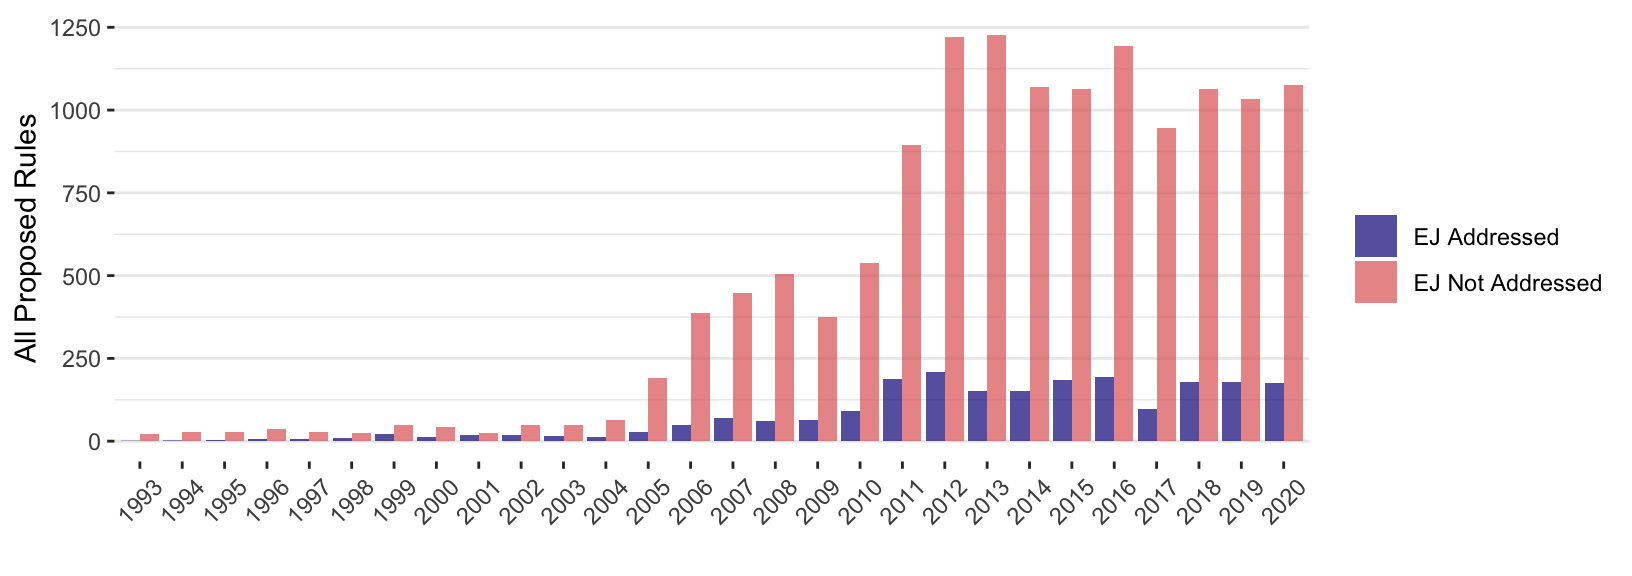
\includegraphics[width=1\linewidth]{/Users/devin/dissertation/Figs/ej-data-ejpr-1} 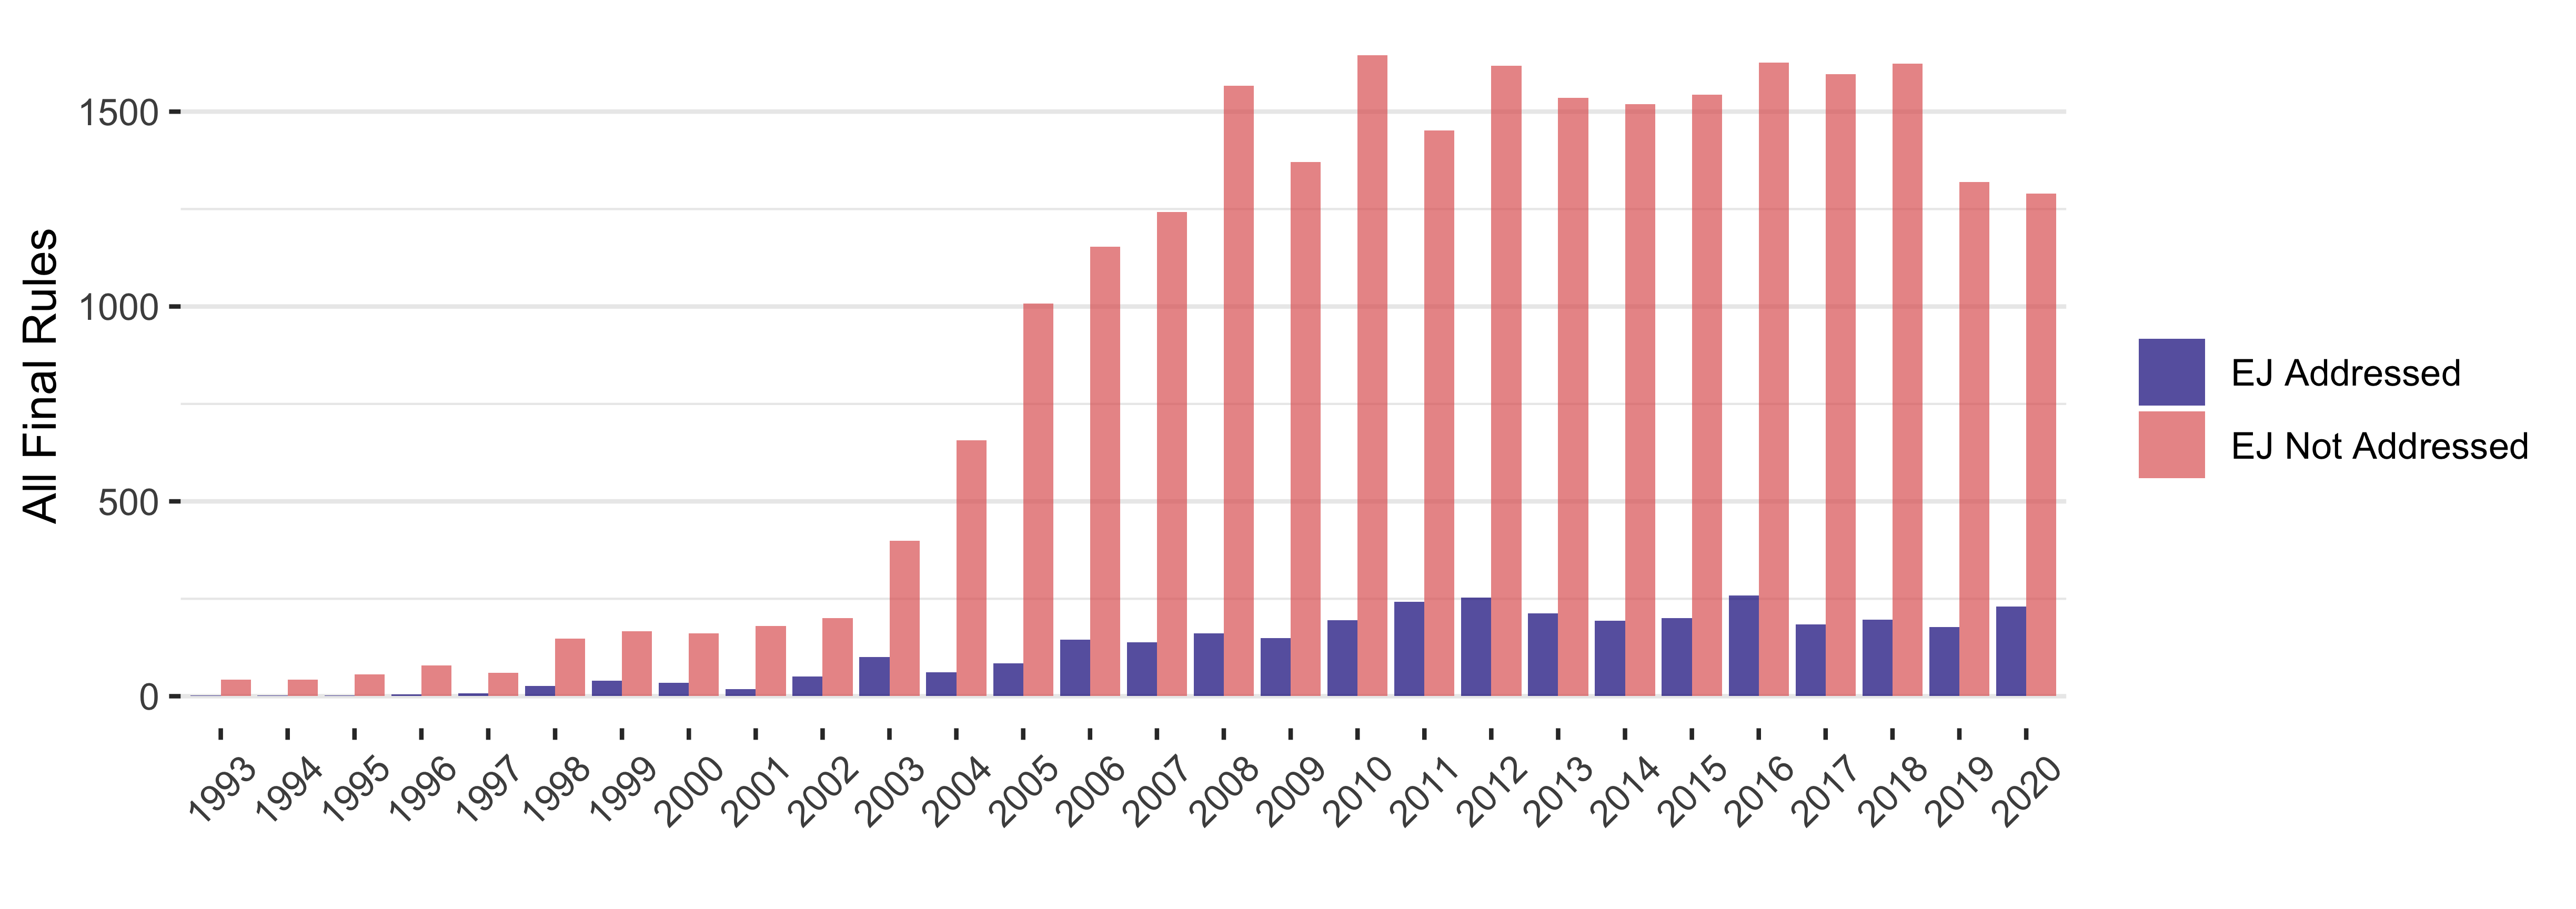
\includegraphics[width=1\linewidth]{/Users/devin/dissertation/Figs/ej-data-ejfr-1} 

}

\caption{Proposed and Final Rules by Whether they Address Environmental Justice.}\label{fig:ej-data}
\end{figure}

Even at the Environmental Protection Agency (EPA), where most policies are clearly framed as ``environmental'' issues, a consistent minority of rules address EJ. Many agencies that make policy with apparent EJ effects almost never address EJ. These include the Fish and Wildlife Service (FWS), Department of Housing and Urban Development (HUD), National Oceanic and Atmospheric Administration (NOAA), Nuclear Regulatory Commission (NRC), and the Office of Surface Mining (OSM). A majority of rules addressed EJ only in a few years at a few agencies that publish relatively few rules, including the Council on Environmental Quality (CEQ), Army Corps of Engineers (COE), Federal Emergency Management Agency (FEMA), Forest Service (FS), and several Department of Transportation agencies (the Federal High Way Administration (FHWA), Federal Motor Carrier Safety Administration (FMCSA), Federal Railroad Administration (FRA), and Federal Transit Administration (FTA)). Figure \ref{fig:ej-data-agencies100} shows the number of rulemaking projects over time by whether they ultimately addressed EJ at agencies that either published more than ten rules addressing EJ or receiving over 100 comments raising EJ concerns.

\begin{figure}

{\centering 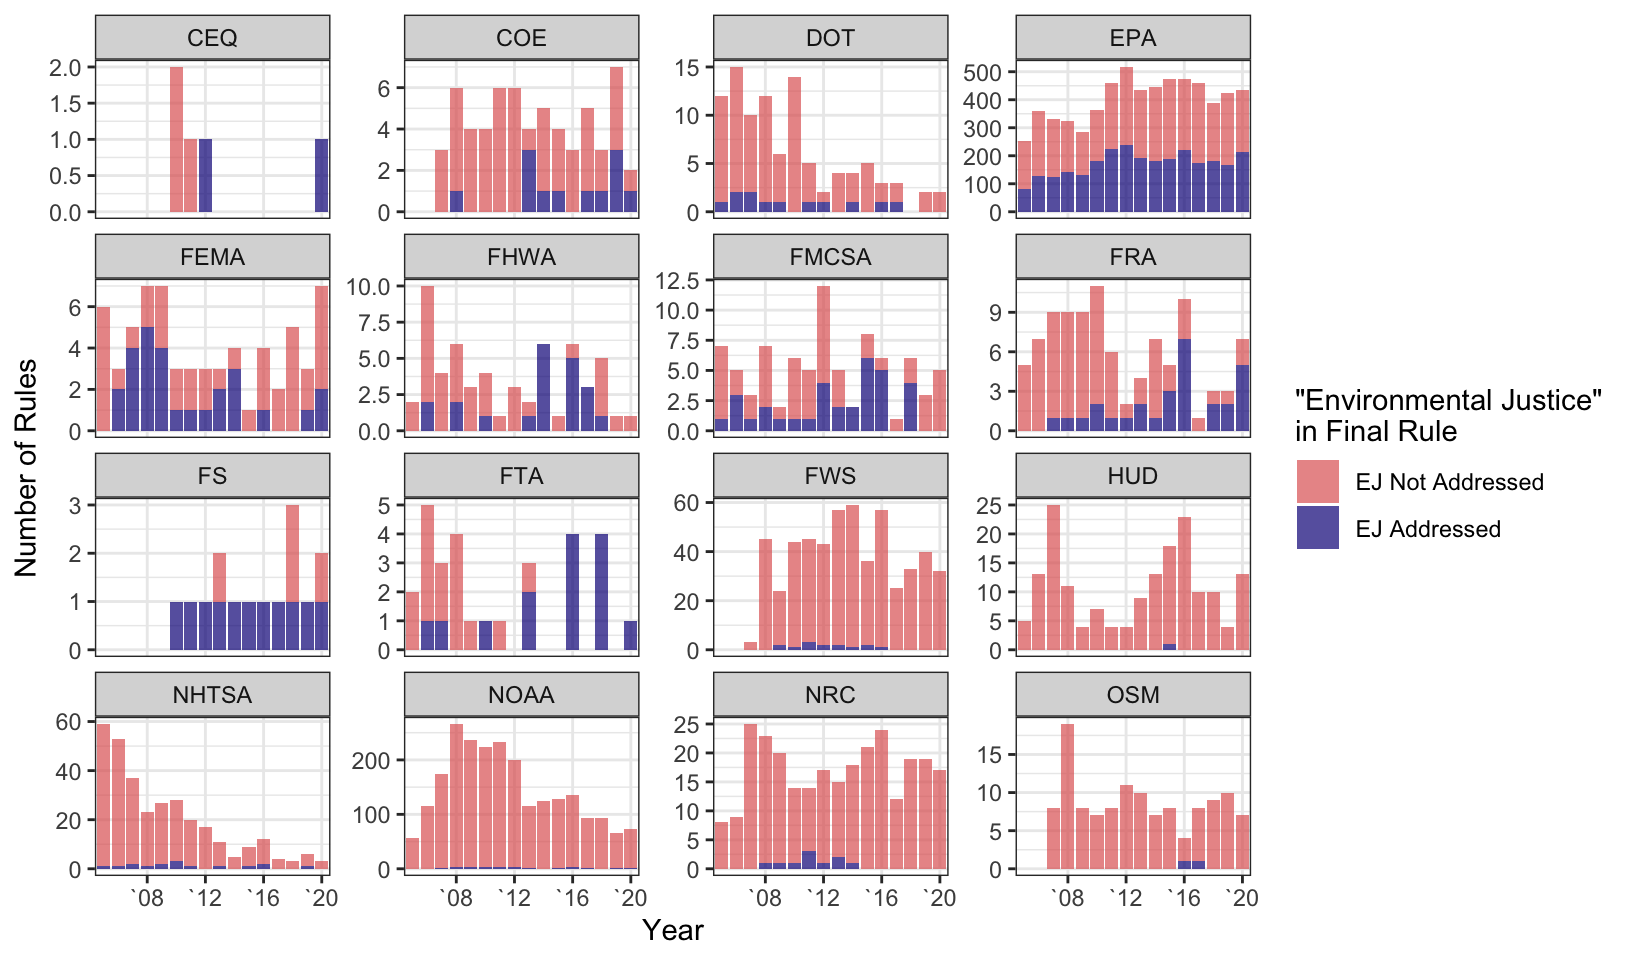
\includegraphics[width=1\linewidth]{/Users/devin/dissertation/Figs/ej-data-agencies100-1} 

}

\caption{Number of Proposed and Final Rules Addressing Environmental Justice at the Council on Environmental Quality (CEQ), Army Corps of Engineers (COE), Department of Transportation (DOT), Environmental Protection Agency (EPA), Federal Emergency Management Agency (FEMA), Federal High Way Administration (FHWA), Federal Motor Carrier Safety Administration (FMCSA), Federal Railroad Administration (FRA), Forest Service (FS), Federal Transit Administration (FTA), Fish and Wildlife Service (FWS), Department of Housing and Urban Development (HUD), National Highway Transportation Saftey Administration (NHTSA), National Oceanic and Atmospheric Administration (NOAA), Nuclear Regulatory Commission (NRC), and Office of Surface Mining (OSM)}\label{fig:ej-data-agencies100}
\end{figure}

\hypertarget{comments}{%
\paragraph{Comments}\label{comments}}

Figure \ref{fig:ej-comments} shows the number of comments on each proposed rule published between 1993 and 2020. Light red circles indicate rules where no commenters raised EJ concerns. Dark blue Triangles indicate rules where they did. The bottom row shows the subset of rules where ``environmental justice'' appeared in neither the draft nor the final rule. The middle row shows rules where ``environmental justice'' appeared in the final but not the draft. My first analysis compares these two subsets. The top row shows rules where ``environmental justice'' appeared in both the draft and final rule. My second analysis assesses change in this subset of rules. Predictably, commenters most often raised EJ concerns on rules in the first row, but many rules that did not initially address EJ still received comments raising EJ concerns.

\begin{figure}

{\centering 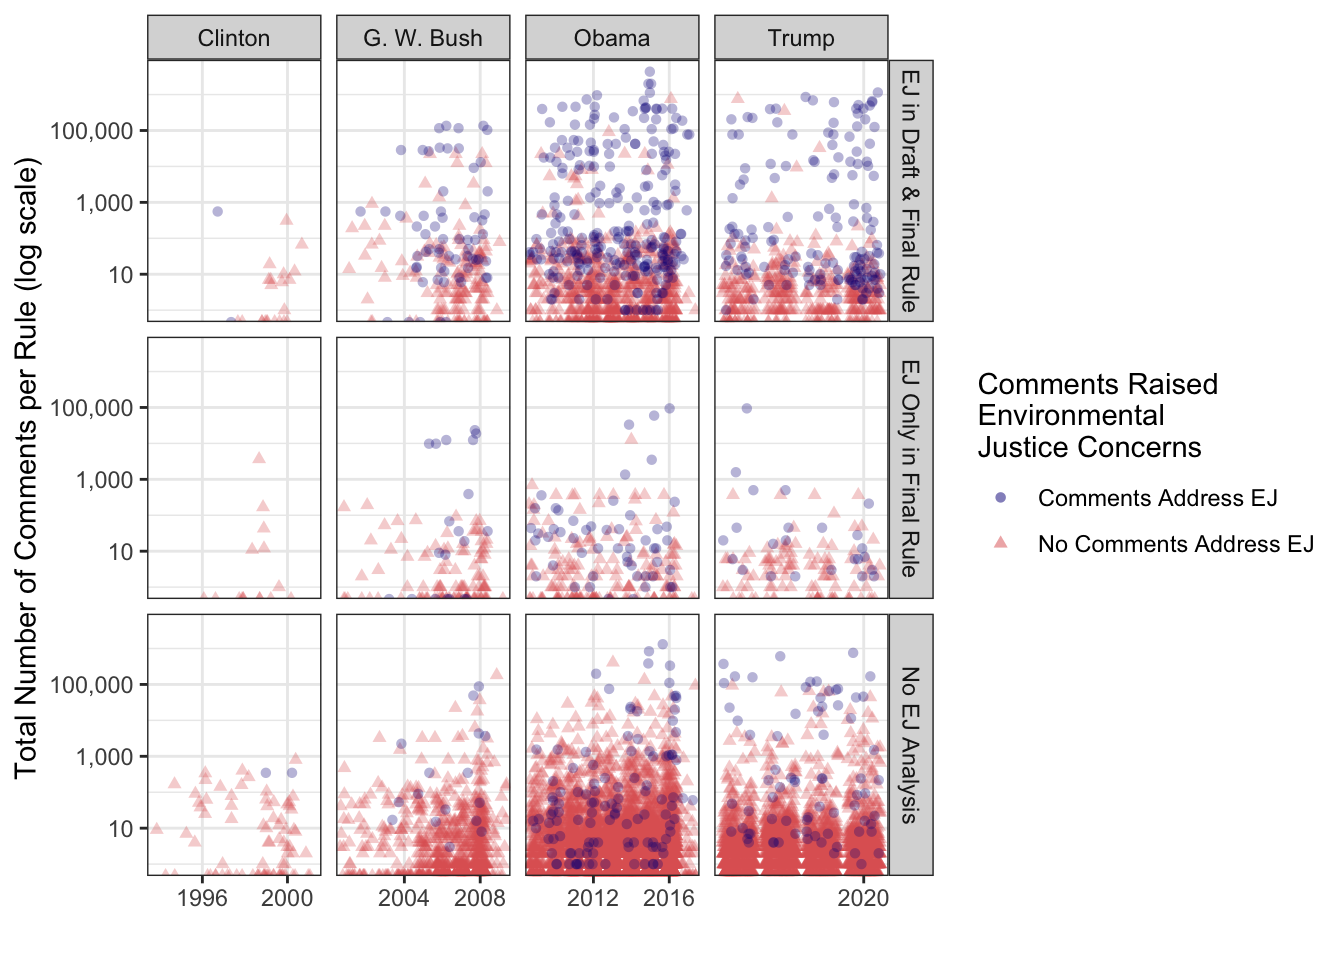
\includegraphics[width=1\linewidth]{/Users/devin/dissertation/Figs/ej-comments-1} 

}

\caption{Number of Comments on Proposed and Final Rules and Whether Comments Raised Environmental Justice Concerns}\label{fig:ej-comments}
\end{figure}

\hypertarget{interest-groups-and-second-order-representation}{%
\paragraph{Interest Groups and Second-order Representation}\label{interest-groups-and-second-order-representation}}

When lobbying during rulemaking, groups often
make dubious claims to represent broad segments of the public \citep{Seifter2016UCLA}. Thus, to interpret substantive results or the normative import of any findings in this analysis, it is insufficient to know which groups participate. We
also need to know who these groups claim to represent and whether those people are actually involved in the organization's decisions.

I examine who is raising EJ concerns in two ways.
First, I identify the top organizational commenters such as tribes,
businesses, and nonprofits using EJ language
and investigate whom these groups represent. Second, for comments where a
commenter signed their name, I compare surnames to their racial and ethnic identity propensities in the U.S. Census. Together these
two pieces of information allow me to comment on ``second-order'' representation, i.e., the extent to which public comments are
representative of the groups they claim to represent \citep{Seifter2016UCLA}.

\hypertarget{which-organizations-most-often-raise-ej-concerns}{%
\subparagraph{Which Organizations Most often Raise EJ Concerns?}\label{which-organizations-most-often-raise-ej-concerns}}

The top mobilizer of comments mentioning ``environmental justice'' between 1993 and 2020 was the Sierra Club, with over 340,000 comments mentioning EJ on dozens of rules. The Sierra Club a membership organization whose members pay dues, elect the leaders of local chapters, and have some say in local advocacy efforts. However, its policy work is directed by a more traditional national advocacy organization funded by donations, including over \$174 million from Bloomberg Philanthropies that funded several of the public pressure campaigns in these data. The Sierra Club does have a major program arm dedicated to Environmental Justice that works with local partners ``to foster the growth of the environmental justice movement so that oppressed communities will find justice and everyone can experience the benefits of a healthy and sustainable future.'' The extent to which those individuals have a formal say in the national organization's lobbying decisions varies across campaigns. The National Board of Directors adopted a statement on social justice in 1993 and principles on environmental justice in 2001. The national website does contain regular Spanish language content. As a federated organization with many local efforts, it is difficult to generalize about second-order representation.

The second most prolific organizer of EJ comments was Earthjustice, with over 175,000 comments on many of the same rules that the Sierra Club lobbied on. Earthjustice is primarily engaged in litigation on
behalf of environmental causes. Their website boasts 2.2 million
supporters, but it is not clear who they are or if they play any role in
the advocacy strategy. A search on the website returns 360 results for
``Environmental Justice,'' with the top results from staff biographies
who work on more local or targeted campaigns, such as environmental conditions
for the incarcerated. The EJ language used on the
main page is relatively vague. For example, ``We are fighting for a future
where children can breathe clean air, no matter where they live.''
\citep{Earthjustice2017}. The website does contain some Spanish language content.

The Natural Resources Defense Council is similar to Earthjustice--a
national nonprofit funded by donations and focused on litigation--but
they also lobby and organize public pressure campaigns, including over 160,000 comments mentioning environmental justice.

CREDO Action and MoveOn are more generic progressive
mobilizers who lack a systematic focus on EJ issues,
but occasionally leverage their vast membership and contact lists to support
EJ campaigns led by others.

The Alliance for Climate Protection is more of an elite political group founded by former Vice President Al Gore.

We Act and Communities for a Better Environment both have environmental
justice in their central mission statement. Community leaders founded We Act in Harlem, New York, to advocate against environmental racism and poor air quality \citep{WEACT2017}. Communities for a Better Environment has projects throughout California but is particularly
active in Oakland \citep{CBECAL2017}. Much of the
content of their website is in both English and Spanish. Both
organizations focus primarily on ``low-income communities of color'' and frame their work primarily in terms of race and class. While both
organizations participated in national policymaking, We Act is more
focused on communities in Harlem and New York, whereas Communities for a
Better Environment casts a broader frame: ``CBE's vision of environmental
justice is global--that's why the organization continues to participate
in such international efforts as the Indigenous Environmental Network
and the Global Week of Action for Climate Justice'' \citep{CBECAL2017}.

While not a large portion of EJ comments, companies repeatedly raise research about the unequal impacts of policy to frame these issues as a legitimate but unresolved scientific debate that is not yet conclusive enough to base regulations on, mirroring the way tobacco and fossil fuel companies have emphasized scientific uncertainty in their lobbying efforts.\textless!-TODO CITE--\textgreater{}
For example, in one comment, the Southern Company wrote:

\begin{quote}
``People with lower SES are exposed to almost an order of magnitude
more traffic near their homes (Reynolds et al., 2001), and live closer
to large industrial sites and are exposed to more industrial air
pollution (Jerrett et al., 2001). Legitimate health concerns must be
addressed. But adopting standards with a scientific basis so uncertain
that health improvement cannot be assured is not sound public health
policy.''
\end{quote}

Like many companies, they claim to represent their customers:
``electric generating companies and their customers are expected to bear
much of the burden'' of regulations \citep{Hobson2004}. Yet, customers have little say in companies' decisions.

Overall, regarding second-order representation, it appears that the groups
most often using the language of environmental justice may do so
sincerely but generally represent affected communities in a surrogate capacity \citep{Mansbridge2003}. Several groups representing local communities and led by community leaders have
participated, but not nearly as often or with the same intensity as the
``big greens.'' The domination of large advocacy organizations highlights the importance of resources as a condition
for lobbying and mobilizing. Not all groups who may benefit from generating political
information can leverage it because they lack the resources to
fund a campaign or even comment on relevant policies. However, smaller, more
member-driven groups may partner with national groups that have more resources to
mobilize on their behalf.
Finally, a third, much less common type of commenter raises EJ issues
to reframe them as ongoing debates and thus undermine their
urgency. I call this reason for engaging an attempt to ``break a perceived
consensus.'' In a way, the fact that energy companies felt compelled to
acknowledge and question EJ concerns suggests their
importance for policy outcomes.

\hypertarget{commenter-race}{%
\subparagraph{Commenter Race}\label{commenter-race}}

To estimate the racial distribution of commenters
using EJ language, I select commenters who
signed with a
surname appearing in census records. Figure
\ref{fig:ejcommentsbyrace} shows a probabilistic racial
distribution of commenters who raise EJ concerns in
their comments based on the distribution of self-reported racial identities
associated with surnames as recorded in the 2010 census.\footnote{I recode ``Hispanic'' as ``Latinx''} I estimate this distribution using the proportion of people with a given surname identified as belonging to each racial
category (from this limited set of options). This approach does not
assign specific individuals to racial categories. Instead, it represents each commenter as a set of probabilities adding up to 1. The estimated racial distribution of the sample is the sum of individual probabilities.

\begin{figure}

{\centering 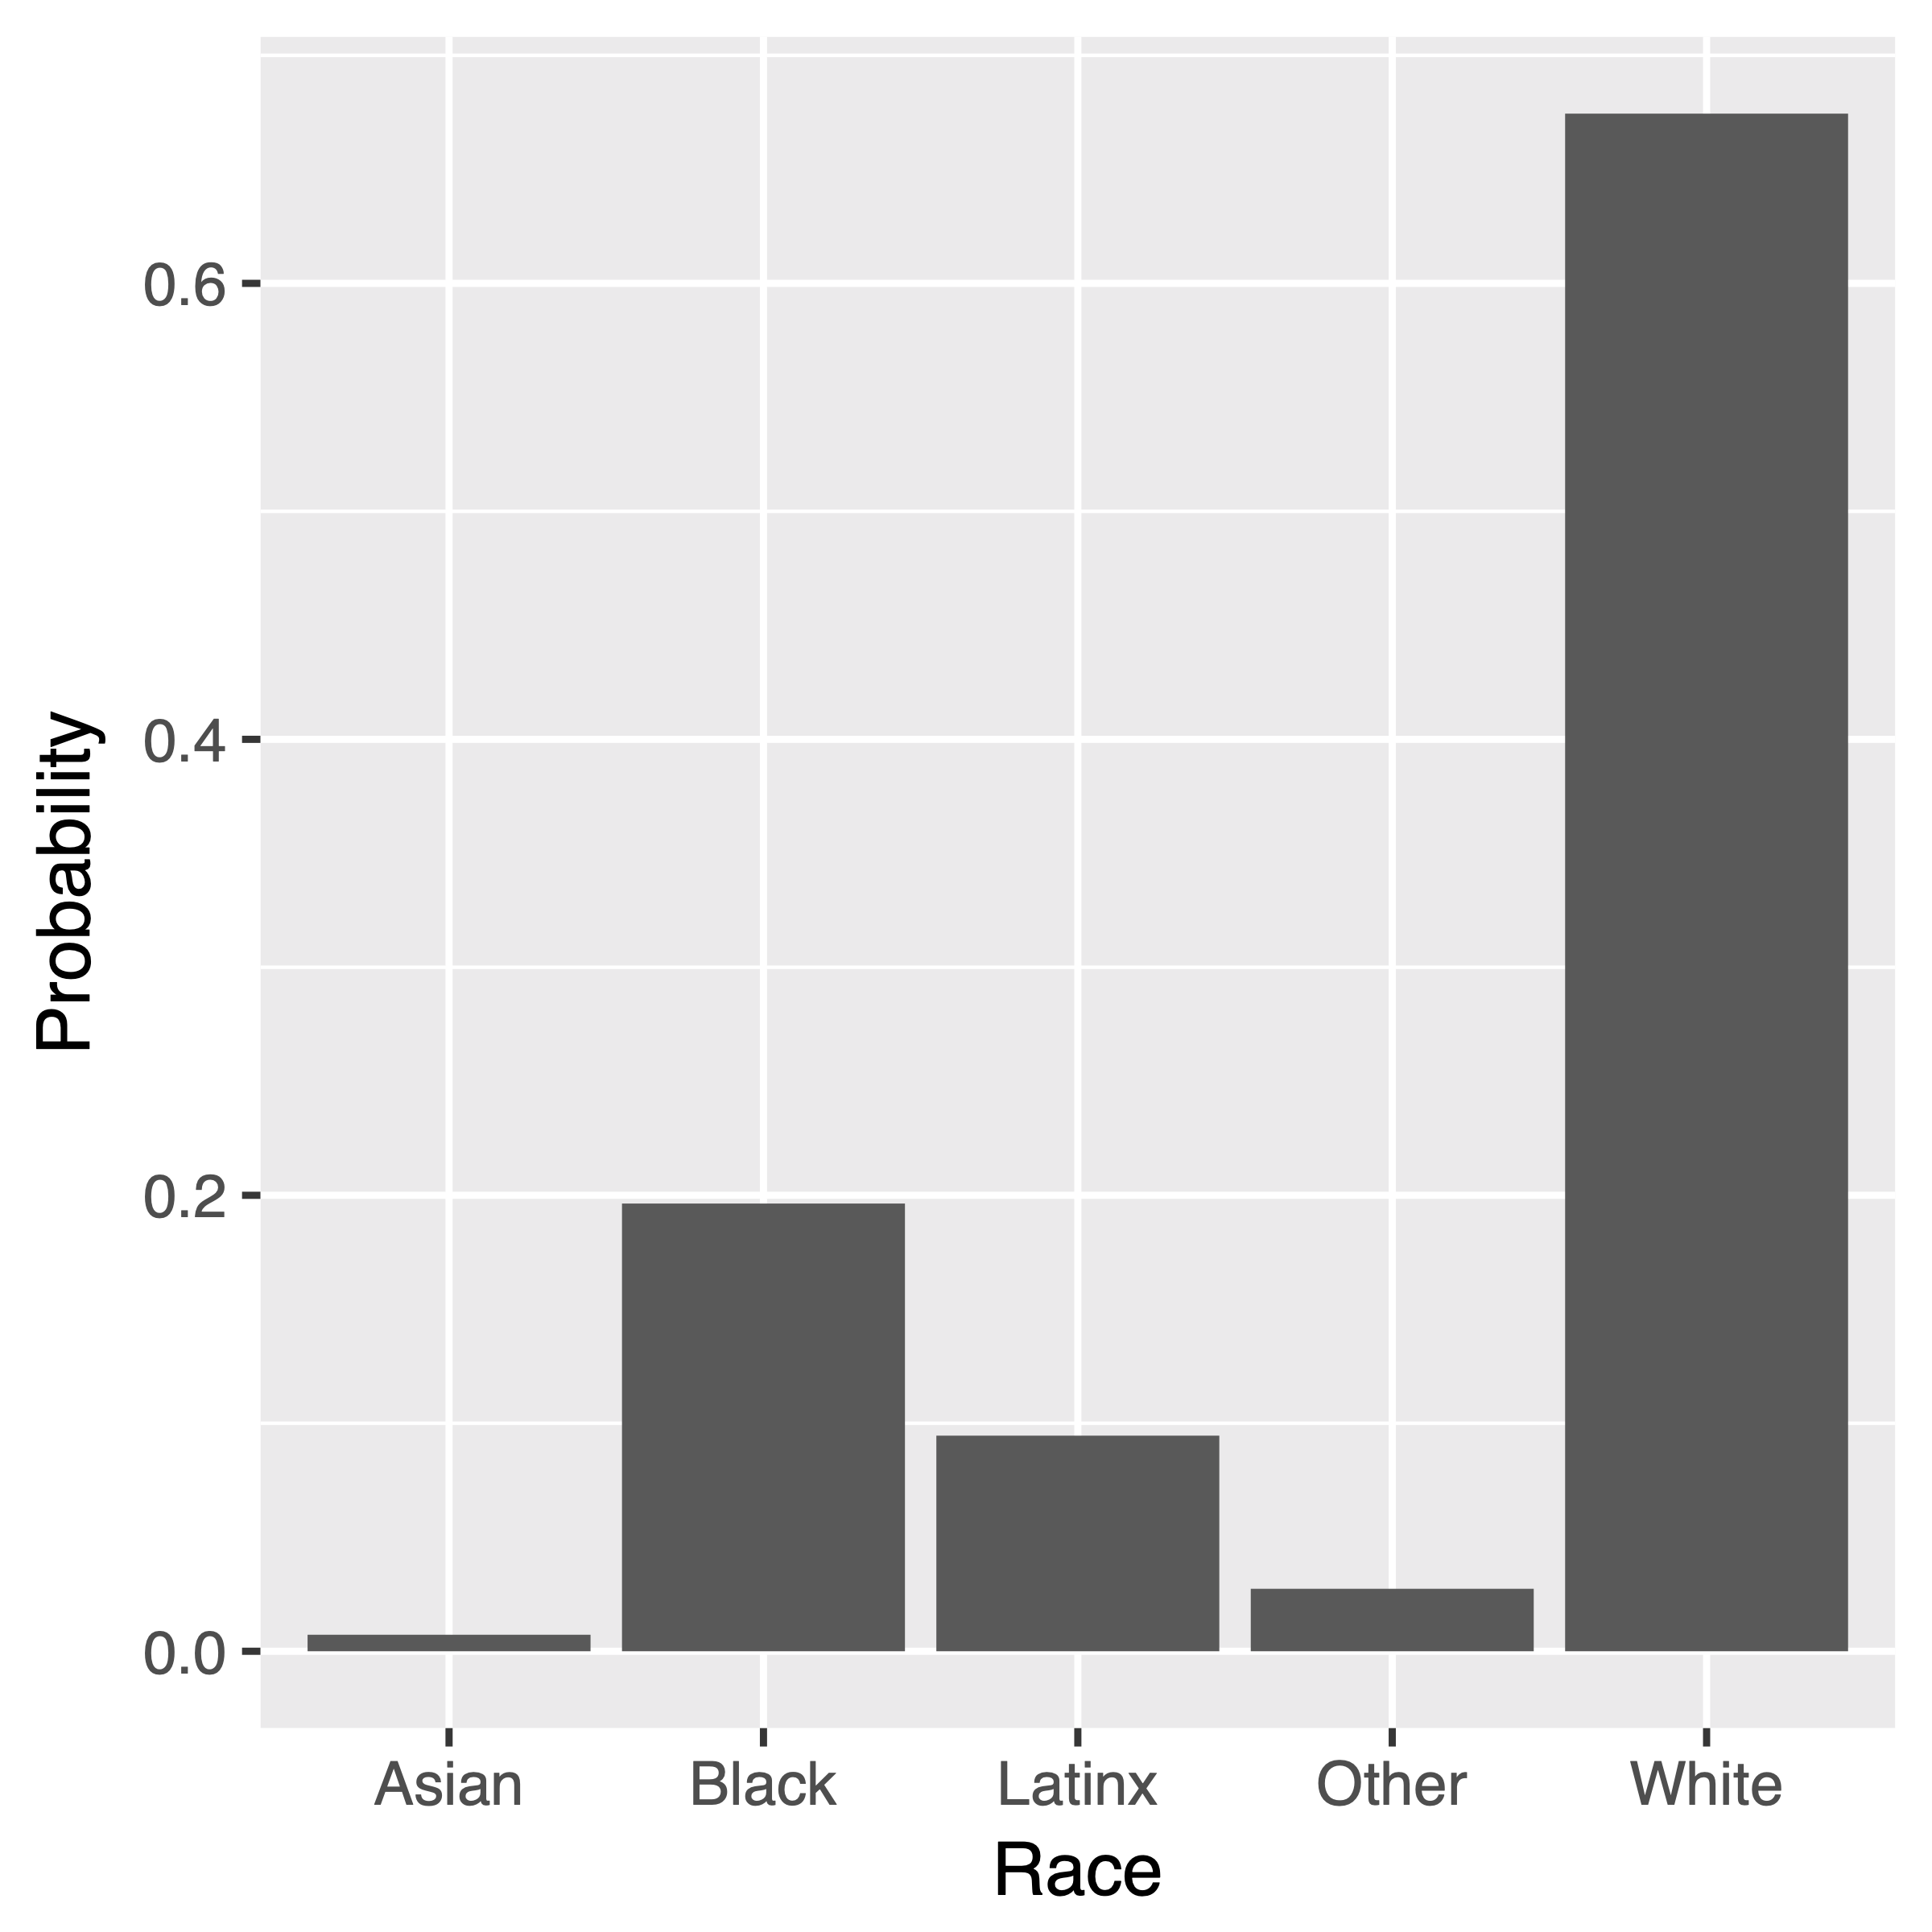
\includegraphics[width=0.49\linewidth]{/Users/devin/dissertation/Figs/race-prob} 

}

\caption{Estimated Racial Distribution from Census Surnames of Commenters raising "Environmental Justice" Concerns in Rulemaking}\label{fig:ejcommentsbyrace}
\end{figure}

Compared to the overall distribution in the 2010 census, this sample of commenters appears to be disproportionately Black and less than proportionately
Latinx or Asian, with just slightly fewer Whites relative to the
national population. This distribution makes sense given that environmental justice
African Americans have led theorizing and activism
\citep{Bullard1993}.

\hypertarget{tracing-ideas-through-rulemaking-environmental-justice-as-a-contested-concept}{%
\subsubsection{Tracing Ideas Through Rulemaking: ``Environmental Justice'' as a Contested Concept}\label{tracing-ideas-through-rulemaking-environmental-justice-as-a-contested-concept}}

Using an environmental justice frame does not always imply the same
communities of concern. Environmental justice emerged from movements
against environmental racism, especially the disposal of toxic
materials in predominantly-Black neighborhoods \citep{Bullard1993}. However, the term
quickly took on other meanings, encompassing various marginalized groups. President Clinton's 1994 Executive Order on
Environmental Justice required all parts of the federal government
to make ``addressing disproportionately high and adverse human health or
environmental effects of programs, policies, and activities on minority
populations and low-income populations'' a core aspect of their mission.
This meant considering disproportionate effects of policies by race and income during rulemaking.

In 2005, Environmental Protection Agency (EPA) political appointees reinterpreted the Order, removing race as a factor in identifying and prioritizing populations. This move was criticized by activists and two reports by EPA's own Office of Inspector General.

President Obama's EPA Administrators reestablished race as a factor. They named EJ as one of their top priorities, but they also faced criticism from activists for paying lip service to environmental racism without adequate policy changes.

In an October 2017 proposed rule to repeal
restrictions on power plant pollution, the Trump EPA acknowledged that
``low-income and minority communities located in proximity to {[}power
plants{]} may have experienced an improvement in air quality as a result
of the emissions reductions.'' Because the Obama EPA discussed
EJ when promulgating the rule, the Trump EPA attempted to reframe rather than ignore environmental justice. The Trump EPA contended that the Obama EPA ``did not address lower household energy bills for low-income households {[}and that{]} workers losing jobs in regions or occupations with weak labor markets would have been most vulnerable'' (EPA 2017). Like regulated industry commenters, these statements frame the distribution of jobs and electricity costs as EJ issues to push back against policies that would equalize the distribution of health impacts from pollution.

The central conflict over the role of race in policy analyses is just one of many conflicts that the environmental justice movement has caused to be fought somewhat on its terms. The next section briefly reviews the decades-long policy fight over regulating Mercury pollution to illustrate how these definitional conflicts shape rules and rulemaking. This case and other examples in this article emerged from reading hundreds of rulemaking documents where agencies did and did not respond to comments raising EJ concerns. Their purpose is to assess whether the cases in the quantitative analysis are plausibly what they appear to be: that changes in rule text are, sometimes, causally related to public comments and that non-changes are cases of agencies disregarding comments, not some accident of the data or measures.
The qualitative reading also confirmed other key assumptions, such as the fact that advocates do, in fact, use ``environmental justice'' when they raise distributional concerns, even on many rules that are not about issues traditionally considered ``environmental.''

\hypertarget{the-evolving-distributional-politics-of-mercury-pollution}{%
\paragraph{The Evolving Distributional Politics of Mercury Pollution}\label{the-evolving-distributional-politics-of-mercury-pollution}}

Definitions of the public good and minority rights are
implicit in most policy documents, including agency rules. The public comment process offers an
opportunity to protest these definitions. Protest is one way that
marginalized groups can communicate opinions on issues to government
officials \citep{Gillion2013}. In the EPA's Mercury Rules, two
definitional issues were decisive. First, as with many forms of pollution,
mercury-emitting power plants are concentrated in low-income and
non-White communities. Second, some populations consume much more
locally-caught freshwater fish, a major vector of Mercury toxicity.
Studies inspired by the political controversy around the Mercury Rules
found high risk among certain communities, including ``Hispanic, Vietnamese, and
Laotian populations in California and Great Lakes tribal populations
(Chippewa and Ojibwe) active on ceded territories around the Great
Lakes'' (EPA 2012). Thus the standards that EPA chooses depend on whom the regulation aims to protect: the average citizen,
local residents, or fishing communities. This decision has disparate
effects based on race and class because of disparate effects based on
geography and cultural practices.

In December 2000, when the EPA first announced its intention to regulate
Mercury from power plants, the notice published in the Federal Register
did not address EJ issues, such as the disparate
effects of mercury on certain populations; it only discussed anticipated impacts in
reference to ``the U.S. population'' (EPA 2000). When the first draft rule
was published, it only discussed the effects of the rule on regulated
entities, noting that

\begin{quote}
``Other types of entities not listed could also be
affected'' (EPA 2002).
\end{quote}

Commenting on this draft, Heather McCausland of
the Alaska Community Action on Toxics (ACAT) wrote:

\begin{quote}
``The amount of methyl-mercury and other bioaccumulative chemicals
consumed by Alaskans (especially Alaskan Natives) could potentially be
much higher than is assumed\ldots{} {[}This could increase{]} the Alaskan Native mortality rate for
babies, which according to the CDC, is 70\% higher than the United States
average. Indigenous Arctic \& Alaskan Native populations are some of
the most polluted populations in the world.
Global transport \& old military sites contaminate us too.''
\end{quote}

By citing the CDC, McCausland's comment provided both technical and distributive information. As allies mobilized, public pressure mounted to address the disparate impacts of mercury levels.
After receiving hundreds of thousands of comments and pressure from
tribal governments and organizations, a revised proposed rule echoed McCausland's
comment noting that

\begin{quote}
``Some subpopulations in the U.S., such as Native
Americans, Southeast Asian Americans, and lower-income subsistence
fishers may rely on fish as a primary source of nutrition and/or for
cultural practices. Therefore, they consume larger amounts of fish than
the general population and may be at a greater risk of the adverse
health effects from Hg due to increased exposure'' (EPA 2004).
\end{quote}

After nearly a million additional public comments, a further revised proposed
rule ultimately included five pages of analysis of the disparate impacts
on ``vulnerable populations'' including ``African Americans,'' ``Hispanic,''
``Native American,'' and ``Other and Multi-racial'' groups (EPA 2011). In the final rule, ``vulnerable populations'' was replaced
with ``minority, low income, and indigenous populations'' (EPA 2012). The EPA
had also conducted an analysis of sub-populations with particularly high
potential risks of exposure due to high rates of fish consumption as well
as additional analysis of the distribution of mortality risk by
race.

Of this second round of comments, over 200 unique comments explicitly raised
EJ issues. The Little River Band of Ottawa Indians
expressed the Tribe's

\begin{quote}
``frustration at trying to impress upon the EPA the
multiple and profound impacts of mercury contamination from a Tribal
perspective. Not to mention the obligations under treaties to
participate with tribes on a `Government to Government' basis. At
present, no such meetings have occurred in any meaningful manner with
EPA Region V, the EPA National American Indian Environmental Office, nor
the State of Michigan's Department of Environmental Quality\ldots Although EPA purported to consider environmental justice
as it developed its Clean Air Mercury Rule, it failed utterly. In this
rulemaking, EPA perpetuated, rather than ameliorated, a long history of
cultural discrimination against tribes and their members'' (Sprague
2011).
\end{quote}

Did comments like these play a role in EPA's changed analysis of
whom Mercury limits should aim to protect?
Given the many potential sources of influence, it may be difficult to
attribute causal effects of particular comments on a given policy.
However, comments may serve as a good proxy for the general mobilization
of groups and individuals around an administrative process, and it is
not clear why the EPA would not address EJ in the first
draft of a rule and then add it to subsequent drafts in the absence of
activist pressure. Electoral politics does not offer an easy
explanation. The notice proposing the Mercury Rule was issued by the
Clinton administration, the same administration that issued the
Executive Order on Environmental Justice, and the subsequent drafts that
did address EJ issues were published by the Bush
administration, which had a more contentious relationship with
EJ advocates, while Republicans controlled both
houses of Congress. The expansion of the analysis from one draft to the
next seems to be in response to activist pressure.

\hypertarget{measuring-policy-change}{%
\subsubsection{Measuring Policy Change}\label{measuring-policy-change}}

Having shown how public comments and pressure can influence policy texts, I assess the general relationship between comments and policy change across all rules. I use two indicators of policy change to model the effect of public comments on policy: \emph{whether} a rule addresses EJ and change in \emph{how} it addresses EJ, i.e., change in portions of the text discussing EJ. Both measures represent a relatively low bar, indicating whether the agency explicitly paid any attention to EJ. This is appropriate given that prior research shows little to no effect of public comments from advocacy groups and little attention to EJ in particular.

Examples in the previous section illustrate how text mentioning ``environmental justice'' might be added or change. Carefully tracing a few rulemaking processes also helped to avoid analytic pitfalls. For example, one case where an agency did an EJ analysis and then appeared not to respond to a comment discussing EJ was, in fact, due to the fact that the commenter included an annotated version of the draft rule their comment, adding only ``no comment'' next to the 12898 section. To correct this, I removed text copied from the proposed rule from comments in pre-processing.

\hypertarget{measure-1-adding-text-addressing-ej-to-final-rules}{%
\paragraph{Measure 1: Adding Text Addressing EJ to Final Rules}\label{measure-1-adding-text-addressing-ej-to-final-rules}}

For the subset of draft rules that did not address EJ, I measure whether agencies added any mention of ``environmental justice'' in the final rule. Such additions usually take the form of an ``E.O. 12898'' section where the agency justifies its policy changes with respect to some concept(s) of environmental justice. The next most common addition occurs in the agency's response to comments, explaining how the rule did not have disparate effects or that they were insignificant.

Agencies may both respond to a comment and add a 12898 section. For example, the EPA responded to several commenters, including Earthjustice, the Central Valley Air Quality Coalition, the Coalition for Clean Air, Central California Environmental Justice Network, and Central California Asthma Collaborative: ``EPA agrees it is important to consider environmental justice in our actions and we briefly addressed environmental justice principles in our proposal.'' As the commenters noted, the EPA had not, in fact, addressed environmental justice in the proposed rule, which approved California rules regulating particulate matter emissions from construction sites, unpaved roads, and disturbed soils in open and agricultural areas. EPA did add a fairly generic 12898 section to the final rule but did not substantively change the rest of the policy.

Less frequently, an agency may explicitly dismiss a comment and decline to add a 12898 section. For example, EPA responded to a comment on another rule, ``One commenter stated that EPA failed to comply with Executive Order 12898 on Environmental Justice\ldots We do not believe that these amendments will have any adverse effects on\ldots minority and low-income populations\ldots Owners or operators are still required to develop SSM plans to address emissions\ldots The only difference from current regulations is that the source is not required to follow the plan'' (71 FR 20445). As these examples illustrate, agencies may add text addressing environmental justice that would not satisfy critics. This measure merely indicates whether the agency engaged with the claims.

Most frequently, agencies neither responded to comments nor added a 12898 section.

\hypertarget{measure-2-changing-text-addressing-ej-in-final-rules}{%
\paragraph{Measure 2: Changing Text Addressing EJ in Final Rules}\label{measure-2-changing-text-addressing-ej-in-final-rules}}

Where draft rules did address EJ, I measured whether a rule changed \emph{how} it discussed ``environmental justice'' between its draft and final publication.\footnote{Occasionally, there is more than one version of a proposed or final rule on a rulemaking docket. Here I opt for an inclusive measure of change that counts change from \emph{any} proposed to \emph{any} final rule. If the change occurred between the first and second draft of a proposed rule, I count it as a change. This best captures the concept of rule change. However, estimates are similar if we only count cases where a change occurred between \emph{every} version of the rule.}
When an agency addresses EJ in the draft rule, it is almost always in a section about how it addressed E.O. 12898. In many cases, much of the text of final rules, including 12898 sections, remain exactly the same between draft and final versions.
To measure change, I parse draft and final rules into sentences and identify sentences containing the phrase ``environmental justice.'' If an agency leaves these sentences unchanged between the draft and final rule and adds no new sentences mentioning EJ, this suggests that the agency did not engage with comments raising EJ concerns.\footnote{An alternative approach would be to parse documents by section and assess whether E.O.12898 sections are identical. Parsing by sentences has three advantages: it is computationally faster, it avoids problems with section numbering and other frustrations with section matching, and it captures attention to EJ outside of this section, especially in the section responding to comments. If an agency is paying attention to EJ issues, sentence matching will likely detect it. However, other measures, such as the percent of EJ sentences changed, the percent of words in a 12898 section that changed, or the change in topic proportions \citep{Judge-Lord2017}, could be useful in future work.}

\hypertarget{results}{%
\subsection{Results}\label{results}}

\hypertarget{are-final-rules-more-likely-to-address-environmental-justice-after-comments-do-so}{%
\subsubsection{Are final rules more likely to address environmental justice after comments do so?}\label{are-final-rules-more-likely-to-address-environmental-justice-after-comments-do-so}}

This subsection presents results from an analysis of draft
rules, comments, and final rules. Descriptively,
where environmental
justice is not addressed in the draft rule, a higher percent of rules add EJ language when comments raise EJ concerns. There is a large difference in the rate of addressing EJ between rules where commenters and did (33\%) and did not raise EJ concerns (4\%). However, in most cases, agencies did not respond at all to these commenters' concerns.

Overall rates of adding EJ in rules without EJ comments decreased over time, leveling out at 3\% during the Obama and Trump presidencies. The rates of adding EJ when commenters did raise these concerns is consistently much higher, but it also decreases over time, from 57\% under G.W. Bush to 26\% under Trump.
EPA had a relatively high baseline rate of change (10\%), which increased to 52\% when comments raised EJ concerns. Most other agencies also added EJ at a higher rate when comments raised EJ concerns; indeed, most agencies almost never do so when comments did not raise EJ concerns.\footnote{More discriptive statistics and figures are available in the online appendix.}

Given differences across presidents, agencies, and the number of comments, I estimate logit regression where the outcome is whether environmental justice was addressed in the final rule (Models 1 and 2 in Table \ref{tab:tables}). The predictors are
whether EJ was addressed in the comments, the number of unique comments addressing EJ, the total number of comments, and the interaction between whether EJ was raised and the total number of comments received. Models 3 and 4 are exactly the same as 1 and 2, except that the outcome is now change in how EJ is discussed (described in the next section). All models include fixed effects for the presidential administration. Models 2 and 4 also include fixed effects for agency. Thus, estimates in Models 1 and 3 include variation \emph{across} agencies, whereas estimates in models 2 and 4 rely on variation \emph{within} agencies. All estimates rely on variation \emph{within} the presidential administration.
All predicted probabilities shown below include agency fixed effects, models 2 and 4.

\begin{table}

\caption{\label{tab:tables}Logit Regression Predicting Change in Rule Text}
\centering
\begin{tabular}[t]{lcccc}
\toprule
  & 1 & 2 & 3 & 4\\
\midrule
Dependent Variable & EJ Added & EJ Added & EJ Changed & EJ Changed\\
\hline
EJ Comment & 3.363*** & 2.414*** & 0.717*** & 0.748***\\
 & (0.221) & (0.240) & (0.243) & (0.246)\\
Log(Comments+1) & 0.068** & 0.232*** & -0.147*** & -0.156***\\
 & (0.028) & (0.036) & (0.032) & (0.033)\\
Unique EJ Comments & 0.005 & 0.227*** & 0.032** & 0.036**\\
 & (0.006) & (0.068) & (0.014) & (0.014)\\
EJ comment*Log(Comments+1) & -0.227*** & -0.226*** & 0.071 & 0.069\\
 & (0.052) & (0.072) & (0.050) & (0.051)\\
\midrule
President FE & X & X & X & X\\
Agency FE &  & X &  & X\\
Num.Obs. & 11721 & 11721 & 1885 & 1885\\
AIC & 3868.6 & 3125.6 & 2180.4 & 2166.5\\
BIC & 3927.5 & 3464.6 & 2224.7 & 2327.2\\
Log.Lik. & -1926.296 & -1516.818 & -1082.192 & -1054.252\\
\bottomrule
\multicolumn{5}{l}{\textsuperscript{} * p $<$ 0.1, ** p $<$ 0.05, *** p $<$ 0.01}\\
\multicolumn{5}{l}{\textsuperscript{} }\\
\end{tabular}
\end{table}

\hypertarget{predicted-probability-of-added-text}{%
\paragraph{Predicted Probability of Added Text}\label{predicted-probability-of-added-text}}

As logit coefficients are not easily interpretable, Figures \ref{fig:ej-m-PR-president-median-1}, \ref{fig:ej-m-PR-comments-agencyFE}, and \ref{fig:ej-m-PR-agency-top} show the predicted probability of a final rule addressing environmental justice when the draft rule did not.

Controlling for average rates of policy change per agency and the number of comments, Figure \ref{fig:ej-m-PR-president-median-1} shows a large difference in the probability of policy change when raising EJ concerns. This supports the ``Distributive Information Hypothesis.'' There is a decrease in rates of adding EJ language after the G.W. Bush Administration, but differences between presidents are small compared to the difference between rules that did and did not see EJ comments. Other variables at their modal values: the EPA, zero additional EJ comments, and one comment total.\footnote{All predicted probability plots below also show probabilities at the modal values for other variables: President Obama, the EPA, zero additional EJ comments, and the median number of total comments (one for models 1 and 2; four for models 3 and 4) unless otherwise specified.}

\begin{figure}

{\centering 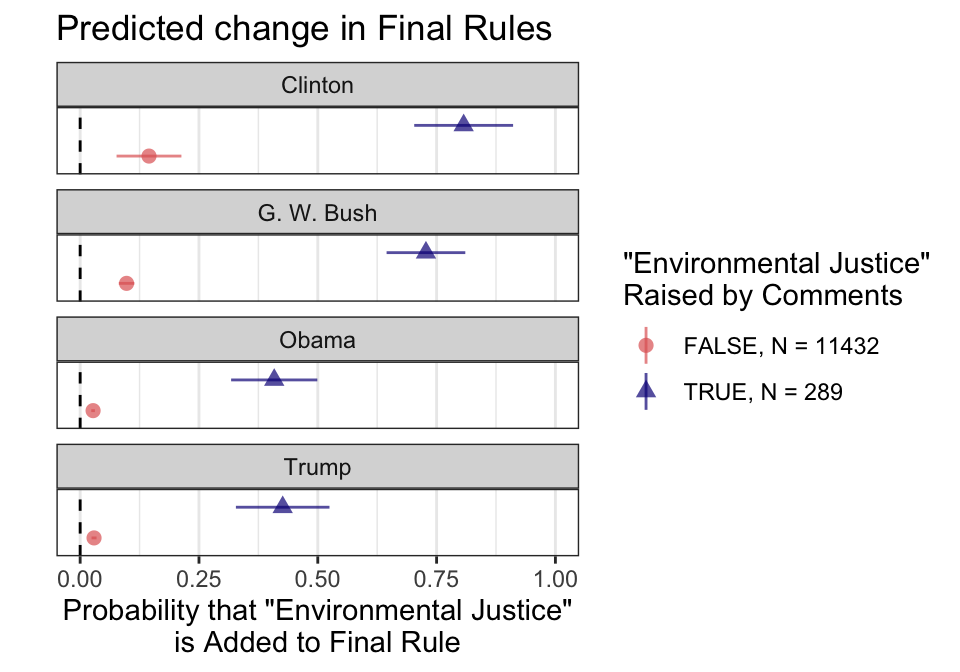
\includegraphics[width=0.8\linewidth]{/Users/devin/dissertation/Figs/ej-m-PR-president-median-1} 

}

\caption{Probability that Environmental Justice is Added Between Draft and Final Rules by President}\label{fig:ej-m-PR-president-median-1}
\end{figure}

Figure \ref{fig:ej-m-PR-comments-agencyFE} shows the probability of EJ language being added with a varying total number of comments.
At low numbers of comments, environmental justice being raised in any one comment does have a decisive relationship with policy change. For rules with less than ten comments (most rules), one comment mentioning EJ is associated with a 30\% increase in the probability that EJ will be addressed in the final rule. This supports the \emph{Distributive Information Hypothesis}. However,
the probability that an agency will add EJ language is still below 50\%---even when comments raise EJ concerns, agencies tend not to address them.

As the number of comments increases, the probability that a rule will add text addressing EJ increases. This supports the \emph{General Pressure Hypothesis}--policy change is more likely when there is more public attention to a policy process. At the same time, there is a negative interaction between the number of comments and EJ comments--the more comments, the smaller the relationship between the comments raising EJ and EJ being addressed in the rule. In the small-portion of highly salient rules with 10,000 or more, the presence of comments raising EJ concerns no longer has a significant relationship with EJ being added to the text. With or without EJ comments, these rules have about the same probability of change as those with just one EJ comment, just under 50\%. This is evidence against the \emph{Specific Pressure Hypothesis}---the number of comments matters (i.e., the scale of public attention) matters regardless of whether these comments explicitly raise EJ concerns. However, as shown in Figure \ref{fig:ej-comments}, very few rules with 10,000 or more comments do not have at least one comment mentioning EJ, so there is a great deal of uncertainty about estimates of the impact of EJ comments with high levels of public attention.

The probability of
``environmental justice'' appearing in the final rule also increases with the number of unique comments that mention ``environmental justice'' in models 2, 3, and 4. Overall this supports the \emph{Repeated Information Hypothesis}.

\begin{figure}

{\centering 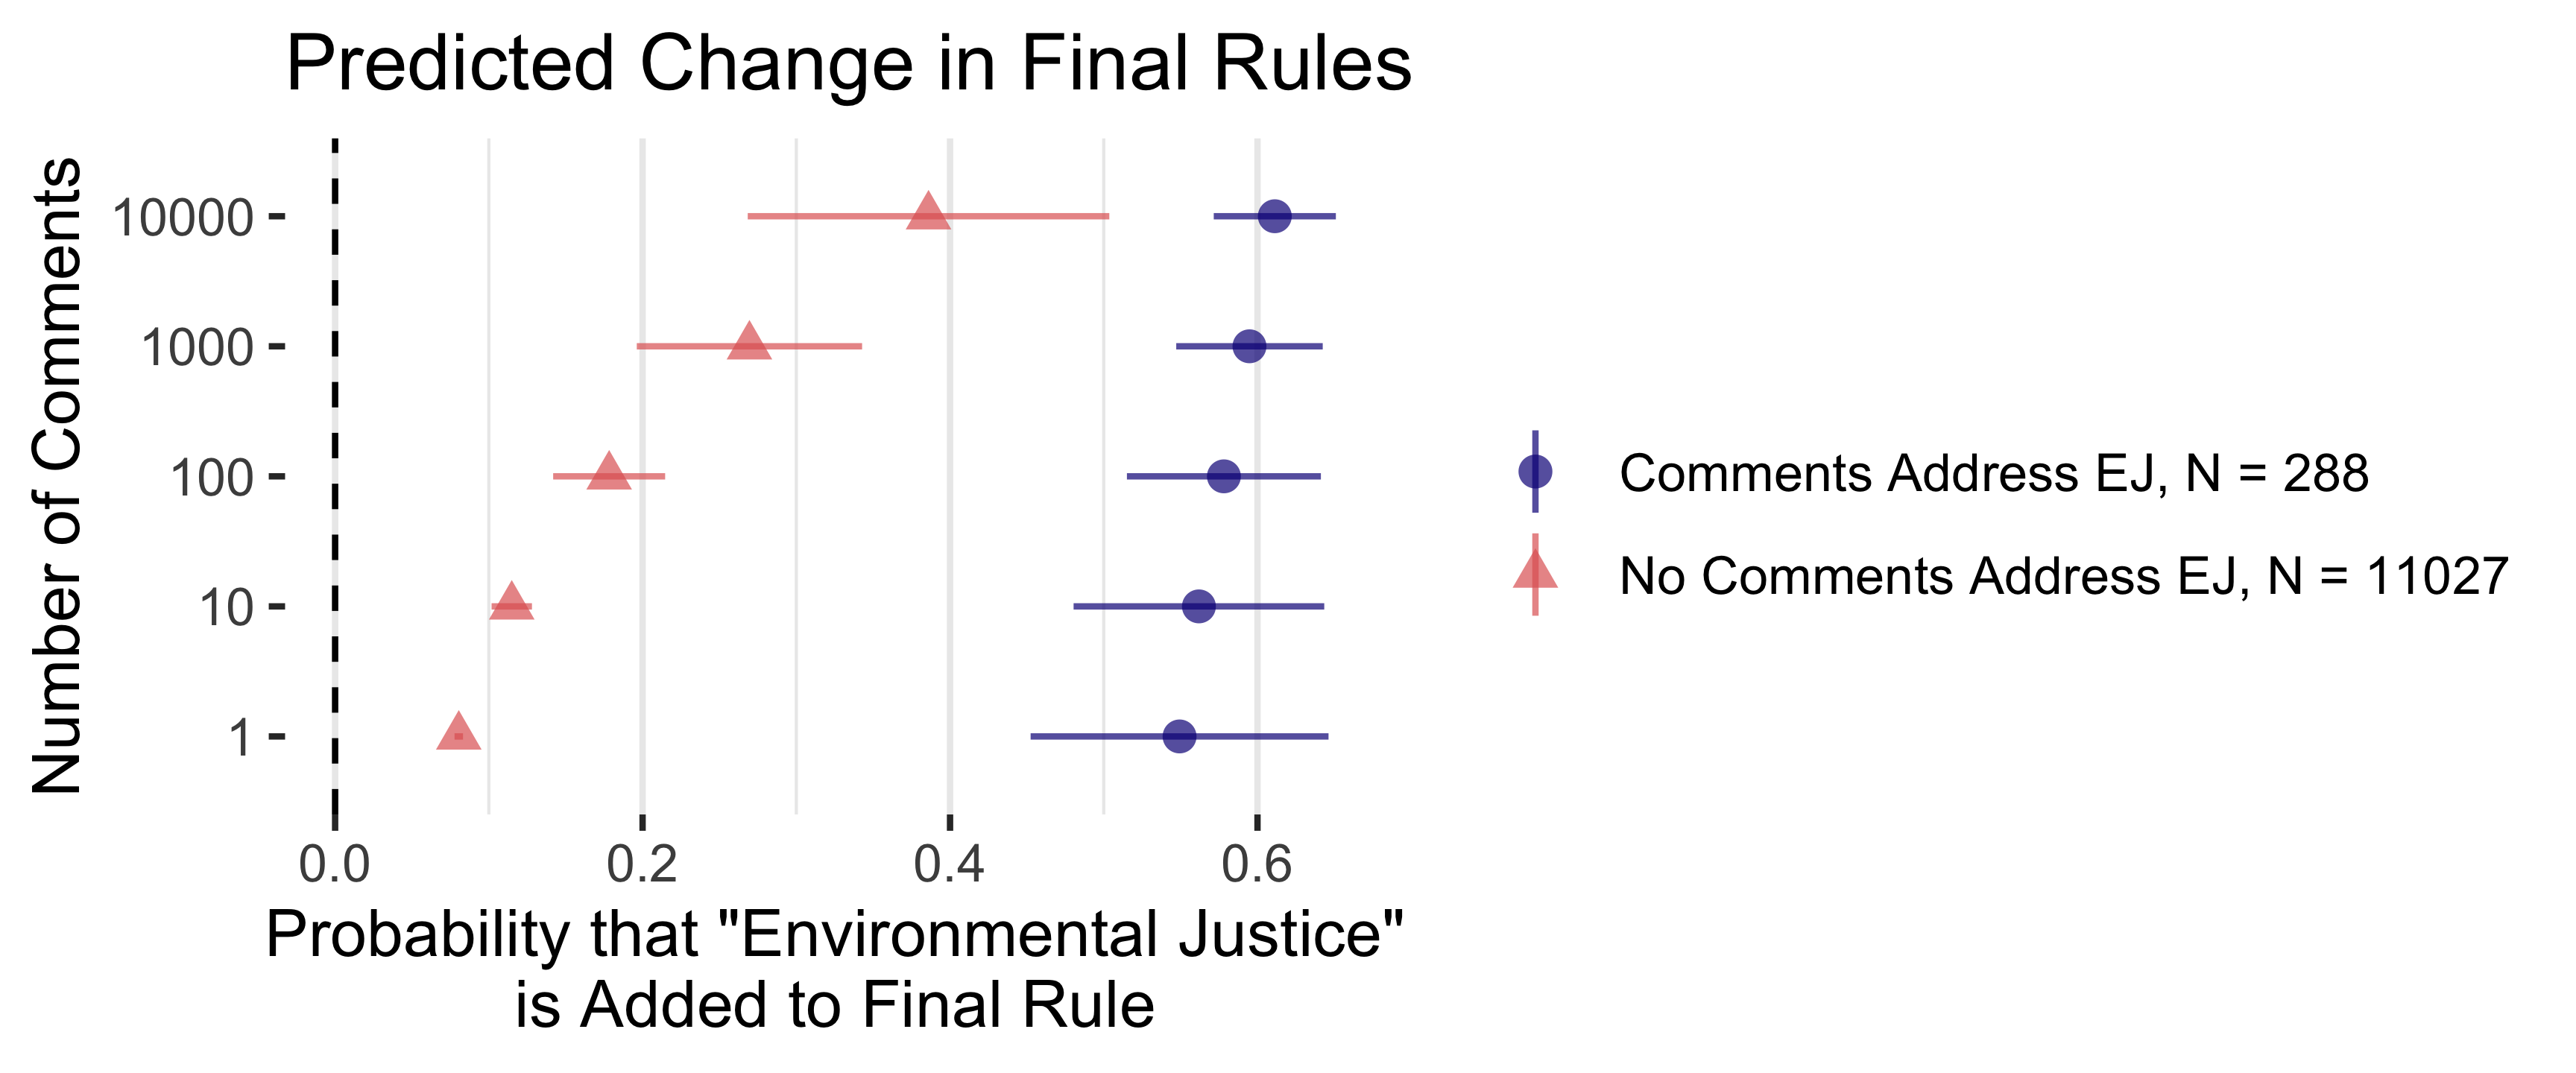
\includegraphics[width=0.8\linewidth]{/Users/devin/dissertation/Figs/ej-m-PR-comments-agencyFE-1} 

}

\caption{Probability Environmental Justice is Added Between Draft and Final Rules by Number of Comments}\label{fig:ej-m-PR-comments-agencyFE}
\end{figure}

Figure \ref{fig:ej-m-PR-agency-top} shows estimated variation in rates of adding EJ to final rules across agencies.
Agencies with the largest average rates of adding EJ language are the agencies we would expect to be more receptive to EJ claims. While many agencies make what could be framed as ``environmental policy,'' and all policy decisions have distributive consequences, institutions have norms and procedures that lead policymakers to see problems in different ways. For example, a few agencies have prominent internal guidance on EJ analysis in rulemaking, including the Environmental Protection Agency and the Department of Transportation (which includes the Federal Railroad Administration (FRA), Department of Transportation, Federal Motor Carrier Safety Administration (FMCSA), and the Federal Highway Administration (FHWA)). However, differences among agencies are fairly uncertain due to the small number of rules where EJ was added at most agencies. Thus, there is more support for the \textbf{Policy Receptivity Hypothesis} than against it, but differences between agencies with different missions and institutional practices regarding EJ is not clear cut.

\begin{figure}

{\centering 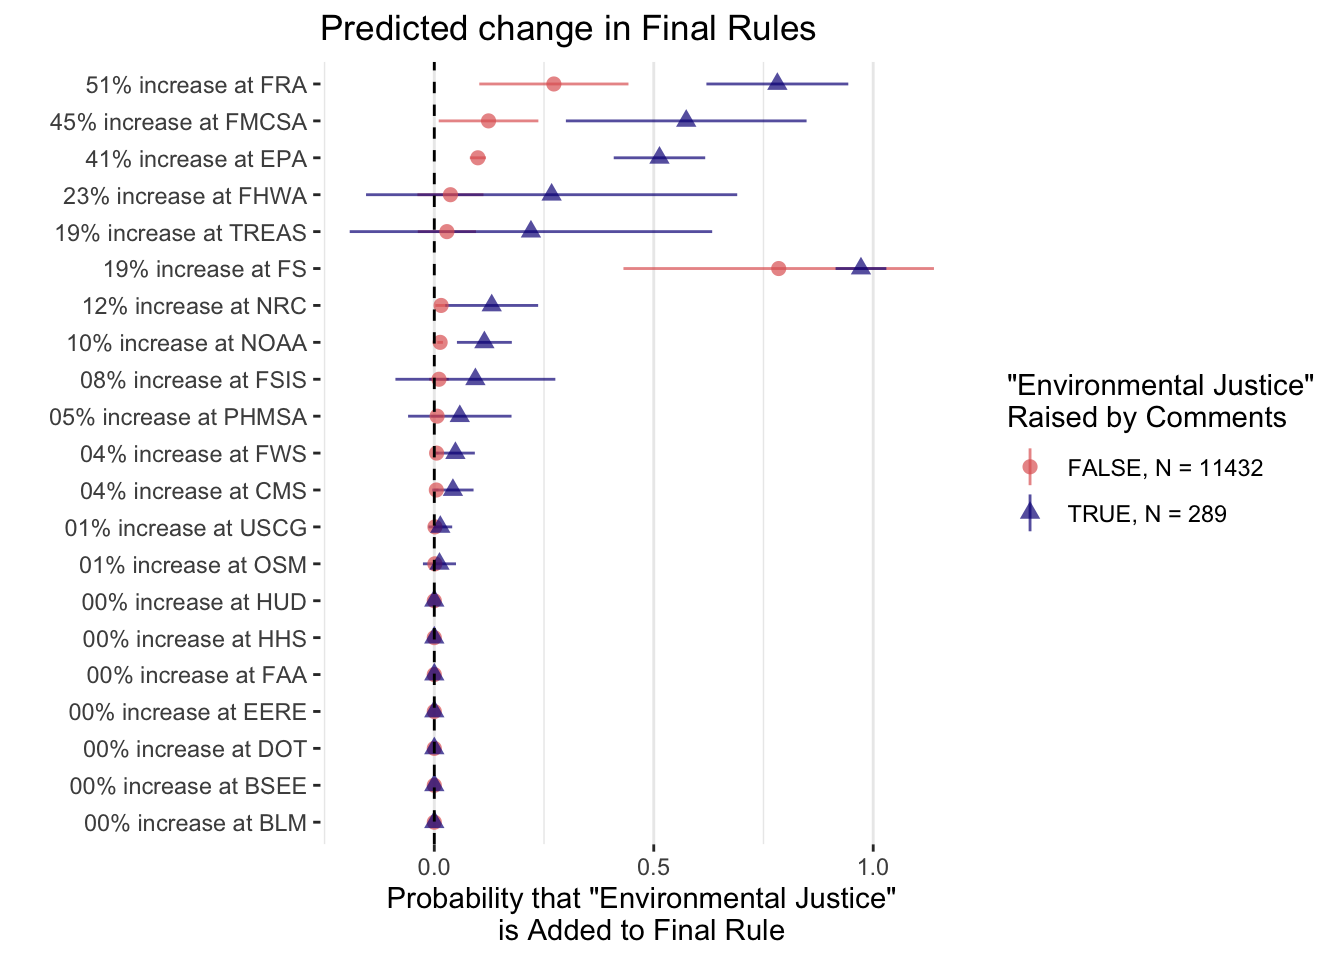
\includegraphics[width=1\linewidth]{/Users/devin/dissertation/Figs/ej-m-PR-agency-top-1} 

}

\caption{Probability Environmental Justice is Added Between Draft and Final Rules by Agency}\label{fig:ej-m-PR-agency-top}
\end{figure}

The Forest Service (FS) has the highest predicted baseline rate of adding EJ to their rules. This may be because the forest service is mainly in
the business of managing forests, leasing timber rights, and controlling
wildfires. These types of decisions have acute distributional
effects. Forest Service rule-writers may also simply have an institutional practice of addressing E.O.12898.
Similarly, the Federal
Railroad Administration, Federal Highway
Administration, Federal Motor Carrier Safety Administration all have large baseline rates of adding EJ to final rules. These agencies are
making decisions about infrastructure projects with implications for
neighborhood environments and air quality. Environmental justice may
often come up.
Research agencies, including the Nuclear Regulatory Commission (NRC), National Oceanographic and Atmospheric Administration (NOAA), also have small but significant baseline rate of adding EJ to final rules.

\hypertarget{are-rules-more-likely-to-change-how-they-address-environmental-justice-when-comments-mention-it}{%
\subsubsection{Are rules more likely to change how they address environmental justice when comments mention it?}\label{are-rules-more-likely-to-change-how-they-address-environmental-justice-when-comments-mention-it}}

Turning to rules that do address EJ in the draft, we also see responsiveness to comments raising EJ concerns, now measured as whether any sentences containing ``environmental justice'' changed between draft and final rule.

Most rules that addressed EJ in the draft were published by the EPA, which had a high rate of baseline change, which increased when comments raised EJ concerns. Other agencies had too few rules to make strong inferences, but many changed how they discussed EJ 100\% of the time when comments raised it, while inconsistently doing so when comments did not.

Models 3 and 4 in Table \ref{tab:tables} are the same as Models 1 and 2, except that the dependent variable is now whether any sentences mentioning EJ changed between the draft and final rule.

\hypertarget{predicted-probability-of-changed-text}{%
\paragraph{Predicted Probability of Changed Text}\label{predicted-probability-of-changed-text}}

Controlling for average rates of change per agency and the number of comments, Figure \ref{fig:ej-mejPR-president-median-1} shows little difference in baseline rates of adding EJ language across the Bush, Obama, and Trump presidencies. All are significantly lower than the rate in the Clinton administration, which could be a result of Clinton's Executive Order or simply an artifact of the limited sample of rules posted to regulations.gov before the mid-2000s.

\begin{figure}

{\centering 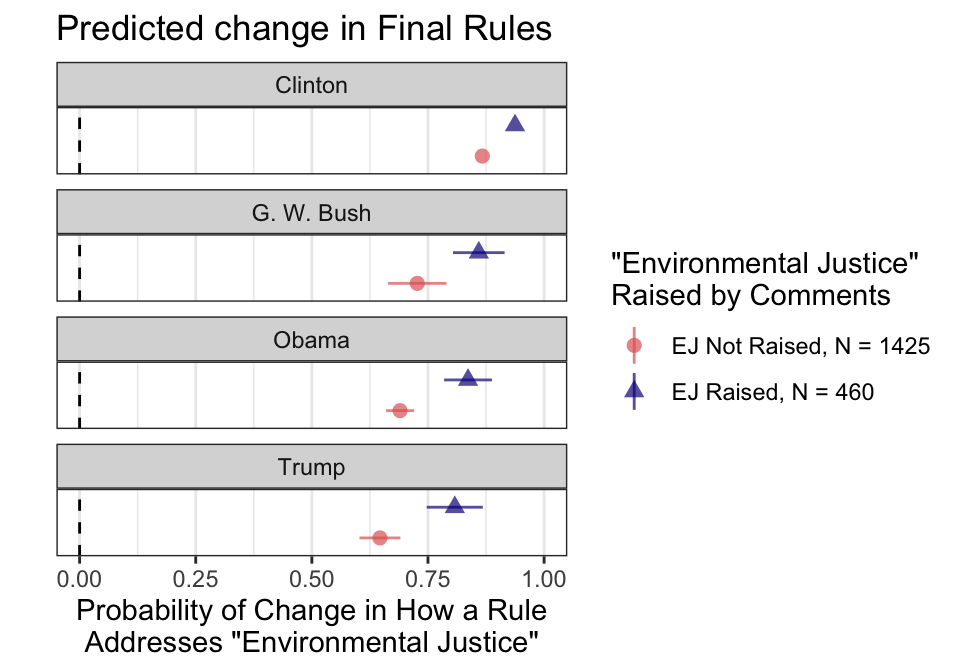
\includegraphics[width=0.8\linewidth]{/Users/devin/dissertation/Figs/ej-mejPR-president-median-1} 

}

\caption{Predicted Change in *How* Environmental Justice is Addressed Between Draft and Final Rules by President}\label{fig:ej-mejPR-president-median-1}
\end{figure}

The relationship between the total number of comments and policy change is in the opposite direction posited by the \emph{General Pressure Hypothesis}. The logged total number of comments has a significantly negative relationship with the probability the final rule text changes. The more comments there are on a proposed rule, the less likely it is to change. Rules are more likely to change when they receive \emph{fewer} comments. The total number of comments thus has the opposite relationship to \emph{how} rules that already addressed EJ changed as it did to \emph{whether} rules added any EJ text. While the \emph{General Pressure Hypothesis} held for adding EJ text, the opposite is true for changing a text that already addressed EJ. Instead, this result supports the competing intuition that more salient rules may be harder to change because the agency has anticipated public scrutiny. Their position set forth in the draft is more likely to be the position of the final rule.

As shown in Figure \ref{fig:ej-mejPR-comments}, EJ comments have a small but discernable relationship to the probability of rule change at typical (low) numbers of comments. As the total number of comments increases, the estimated difference between policies that did and did not receive EJ comments increases. When no comments mention EJ, a rule that receives 10,000 comments is much less likely to change than a rule that received 10,000. When comments do raise EJ concerns, more public attention has a smaller impact on the probability of policy change.

\begin{figure}

{\centering 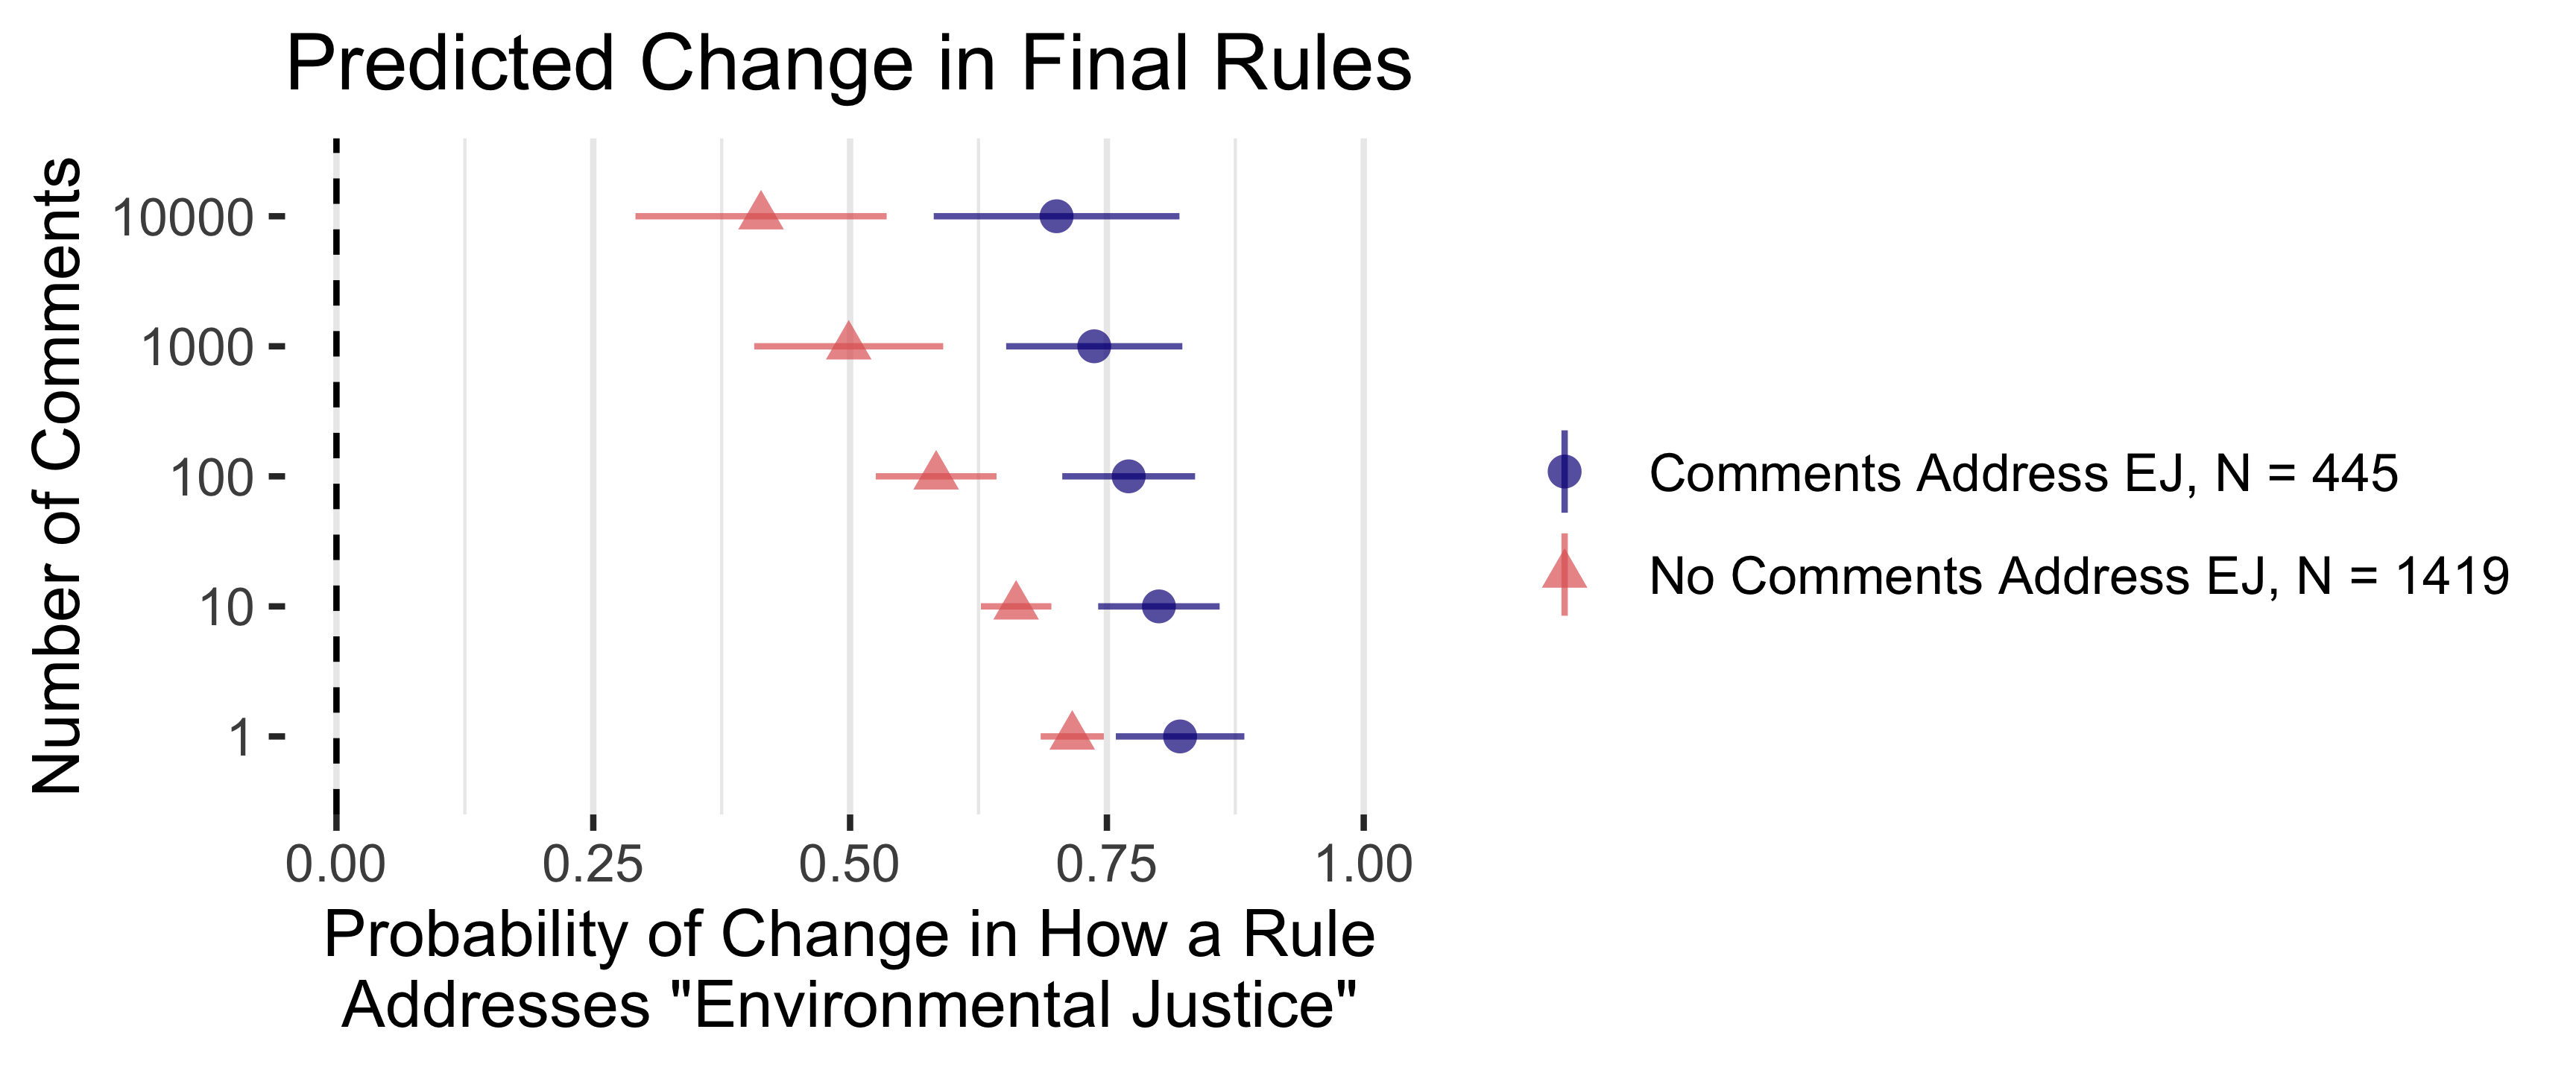
\includegraphics[width=0.8\linewidth]{/Users/devin/dissertation/Figs/ej-mejPR-comments-1} 

}

\caption{Predicted Change in *How* Environmental Justice is Addressed Between Draft and Final Rules by Number of Comments}\label{fig:ej-mejPR-comments}
\end{figure}

\hypertarget{conclusion}{%
\subsection{Conclusion}\label{conclusion}}

The above analysis offers a rare, systematic account of a social movement's impact on specific policy outcomes across institutions and over time. It illustrates the importance of ideas in policymaking and how social movements can affect policy, even in technocratic processes like rulemaking, where most U.S. law is now made.

When activists raise issue frames
like environmental justice, there is a higher probability that
policymakers engage in discourse that highlights the distributive effects of policy. However, baseline rates of addressing environmental justice in rulemaking are so low that, even when activists raise EJ concerns, most policy documents pay no explicit attention to EJ. We see this general lack of attention across agencies and across the G.W. Bush, Obama, and Trump administrations. Indeed, there are surprisingly small differences across administrations in both baseline rates of considering EJ and the relationship between public pressure and policy change.
There is a great deal of variation across agencies, suggesting that policy receptivity and responsiveness to public input are conditional on an
institutional factors.

The policy outcomes suggested by an environmental justice analysis depend on how the populations of concern are defined. In some cases, those raising environmental justice concerns
present it as an issue of wealth or income inequality, leading policy to
account for disparate impacts on low-income populations. In other cases,
groups raise claims rooted in cultural practices, such as fish
consumption among certain tribes. As occurred in the Mercury Rule, the
analysis in subsequent drafts of the policy used evaluative criteria
specific to these communities. Thus, policy outcomes
will depend on the specific environmental justice concerns raised.

Which communities and concerns are raised by activist campaigns depend on second-order representation in the organizations that mobilize public pressure. Examining which groups raise environmental justice concerns and second-order participation in these organizations' advocacy decisions validates some of the skepticism about who is able to
participate and make their voice heard. Elite groups dominate policy lobbying, even for
an issue like environmental justice. National
advocacy organizations frequently request that regulators protect
``all people'' or even ``low-income communities of color.'' However, this
more generic advocacy may not lead to the same outcomes as groups that present more specific local environmental justice concerns unique to a community. In between generic progressive advocacy organizations
and community-based organizations are high-capacity organizations like the Sierra Club and Earthjustice, which frequently partner with local organizations for more place-based litigation and campaigns and may be more likely to raise these local concerns in
national policymaking. Given the importance of federal policy for local environmental outcomes, and advocacy organizations' potential to draw policymakers' attention to environmental justice issues, future research should examine the quality of partnerships between frontline communities and national advocacy organizations.

In the end, the above analysis offers some clarity on two poorly
understood and rarely linked features of American politics: the policy impact of social movements and the role of public pressure in bureaucratic policymaking. It offers
some hope that policymakers may address concerns raised through direct democracy
mechanisms like public comment periods. At the same time, it highlights how policymakers rarely explicitly address the disparate impacts of policy, even when directly confronted with distributive justice concerns. Social movements do affect policy, but there are steep odds to overcome.
% --- PAGE: endnotes -----------------------
% --- PAGE: refs -----------------------
\newpage
\singlespacing 
          \bibliography{/Users/devin/dissertation/assets/dissertation.bib} 
   

\end{document}
